\documentclass[11pt,letterpaper]{article}

\usepackage{showlabels}
\usepackage{fullpage}
\usepackage{pslatex}
\usepackage[english]{babel}
\usepackage[utf8]{inputenc}
\usepackage{amsmath}
\usepackage{bm}
\usepackage{xcolor}
\usepackage{url}
\usepackage{rotating}
\usepackage{natbib}
\usepackage{amssymb}
\usepackage{lingmacros}


%\usepackage{linguex}
%\usepackage{lingmacros}

\usepackage{CJKutf8}
\newcommand{\korean}[1]{\begin{CJK}{UTF8}{mj}#1\end{CJK}}

\usepackage{tikz}


\usepackage{colortbl}

%\usepackage{xeCJK}

\usepackage{natbib}
\bibliographystyle{unsrtnat}

%\usepackage{latexsym}
\usepackage[english]{babel}
\usepackage[utf8]{inputenc}
\usepackage{bm}
\usepackage{graphicx}
%\usepackage{tikz}
\usepackage{xcolor}
\usepackage{url}
%\usepackage[colorinlistoftodos]{todonotes}
\usepackage{rotating}
\usepackage{multirow}




\usepackage{hyperref}

\usepackage{tikz-dependency}
\usepackage{changepage}
\usepackage{longtable}


\newcommand{\R}[0]{\mathbb{R}}
\newcommand{\Prob}[0]{\mathbb{P}}
\newcommand{\Ff}[0]{\mathcal{F}}

\usepackage{multirow}

\newcommand{\soft}[1]{}
\newcommand{\nopreview}[1]{}
\newcommand\comment[1]{{\color{red}#1}}
\newcommand\mhahn[1]{{\color{red}(#1)}}
\newcommand\becky[1]{{\color{blue}(#1)}}
\newcommand\note[1]{{\color{red}(#1)}}
\newcommand\jd[1]{{\color{red}(#1)}}
\newcommand\rljf[1]{{\color{red}(#1)}}
\newcommand{\key}[1]{\textbf{#1}}

\DeclareMathOperator*{\argmax}{arg\,max}
\DeclareMathOperator*{\argmin}{arg\,min}
\DeclareMathOperator{\E}{\mathop{\mathbb{E}}}



%\usepackage{lingmacros}
%\usepackage{linguex}


\usepackage{amsthm}

\newcommand{\thetad}[0]{{\theta-d}}
\newcommand{\thetal}[0]{{\theta-{LM}}}

\newcounter{theorem}
\newtheorem{proposition}[theorem]{Proposition}
\newtheorem{thm}[theorem]{Theorem}
\newtheorem{corollary}[theorem]{Corollary}
\newtheorem{question}[theorem]{Question}
\newtheorem{example}[theorem]{Example}
\newtheorem{defin}[theorem]{Definition}
\newtheorem{definition}[theorem]{Definition}
\newtheorem{lemma}[theorem]{Lemma}


%\usepackage{linguex}
%\newcommand{\key}[1]{\textbf{#1}}



\renewcommand{\thefigure}{S\arabic{figure}}
\renewcommand{\thetable}{S\arabic{table}}
\renewcommand{\thesection}{S\arabic{section}}

\newcommand{\utterance}{\mathcal{U}}
\newcommand{\tree}{\mathcal{T}}



\usepackage{siunitx}



\usepackage{longtable}



\frenchspacing
%\def\baselinestretch{0.975}

%\emnlpfinalcopy
%\def\emnlppaperid{496}

\title{Morpheme Ordering across Languages reflects optimization for Memory Efficiency}

\begin{document}

\maketitle

\begin{abstract}
The order of morphemes in a word shows well-documented tendencies across languages.
Previous work has explained these in terms of notions such as semantic scope and relevance.
A recent theory argues that word and morpheme order in language optimizes a tradeoff between Memory and surprisal, and provided initial evidence from two languages that morpheme order can partly be explained by optimization for this treadeoff.
In this work, we test this idea more extensively using data from four additional agglutinative languages with significant amounts of morphology, in both verb and noun inflection.
We find that the memory-surprisal tradeoff predicts order in most cases with high accuracy.
We also find that it accounts for several, previously documented, universal properties, such as the relative order of number and case suffixes on nouns.
Our work adds to a growing body of work suggesting that many properties of language arise from cognitive principles.
\end{abstract}


\section{Introduction}

Across languages, words are composed of morphemes, commonly defined as the smallest meaning-bearing units of language.
Morphemes can take different shapes.
In many cases, words can be segmented into a sequence of morphemes, as in the English word runners (root run-, derivation -er-, plural -s).
The order of morphemes within a word follows well-documented cross-linguistic tendencies, for instance, plural markers tend to be closer to noun stems than case markers \citep[112]{greenberg1963universals}.
These tendencies have been explained in terms of the relative scope of different morphemes  \citep{rice2000morpheme}, parallelism between morphology and syntax \citep{givon1971historical,venneman1973explanation,baker1985the}, and the strength of their semantic association with the root \citep{bybee-morphology-1985}.
%One family of explanations holds that those affixes are closest to the root that are most relevant to the root \citep{bybee-morphology-1985}.
%Other explanations suggest that morphemes are ordered based on (TODO CITE).

A recent theory proposes a cognitive explanation for these tendencies, arguing that ordering universals in language can be understood as arising from optimization of processing effort under memory limitations \citep{Hahn2020modeling}.
Formally, they introduced the notion of a memory-surprisal tradeoff: Depending on how many memory resources a comprehender invests, they can achieve different levels of surprisal.
(CITE) hypothesize that order of words and morphemes in language optimizes this tradeoff.
Optimizing the memory-surprisal tradeoff amounts to putting elements together when they predict each other strongly, as measured by mutual information.
In a case study, CITE apply this to morpheme ordering in Japanese and Sesotho, finding that optimization could partly reproduce morpheme ordering in these languages.
They also suggested that mutual information formalizes previous notions of strength of semantic association, such as \cite{bybee-morphology-1985}'s notion of \textit{relevance}.






In this work, we examine this theory on a broader basis by considering data from four additional languages.
We focus on languages where words tend to have multiple morphemes and these are mostly realized separately. Such languages are referred to as agglutinative (Greenberg 1954).
We obtained data from four languages (Korean, Turkish, Hungarian, Finnish).
Whereas \cite{Hahn2020modeling} only considered verb inflection, we also consider noun inflection across three languages.


%Greenberg 1963:  "the expression of number almost always comes between the noun base and the expression of case" (Greenberg 1963:112)

%Scope, Syntax, History
%Another family of explanations holds that morpheme ordering is to be explained diachronically, and that morpheme order reflects the order of independent words in earlier stages of a language.
%- Relevance, Proximity Principle, Iconicity




%Bybee on explanation:
%- regarding the historical explanation (Givon 1971, Vennemann 1973):
%Morphology is not always fossilizes syntax (Bybee and Brewer 1980, Bybee 1985 p. 39--40)


\section{Locality and the Memory--Surprisal Tradeoff}

A long line of work in linguistics has proposed principles of locality to account for word order regularities within and across languages (CITE).
An early example is \citep{behaghel1932deutsche}, who argued that elements that are closer together in meaning are closer together in form.
In word order, the Head Proximity principle of \citep{rijkhoff-word-1986} states that words are close to their syntactic heads, and this generalization has since found strong empirical support from data in many languages~\cite[e.g.][]{liu2008dependency, futrell-large-scale-2015-1, liu-dependency-2017}.
In morpheme ordering, \citep{bybee-morphology-1985} argues that morphemes are closer to the root when they are more relevant to it.
One explanation of such principles is in terms of iconicity in form-meaning correspondence \citep{givon1985iconicity}.
More recently, locality principles have been explained in terms of memory and efficiency in online processing \citep{hawkins-efficiency-2003}.
Based on considerations of memory limitations, \citet{futrell2020lossy} derived an information-theoretic locality principle that states that words are close to each other when they are highly predictive of each other (see also \citet{culbertson2020from}).
This principle of information locality TODO


\citet{Hahn2020modeling} proposed a cognitive principle that aims to unify and formalize these locality principles in the form of a Memory--Surprisal Tradoff.
This is a cognitive account of the order of words and morphemes in human language, based on a formalization of memory efficiency in incremental processing.
The memory-surprisal tradeoff links information-theoretic models of memory limitations with surprisal theory.

Surprisal theory \citep{hale2001probabilistic, levy2008expectation} is a theory of the word-by-word processing difficulty in online processing.
It states that the processing effort on a word $w_t$ in context $w-1 ... w_{t-1}$ is proportional to its surprisal
     \begin{equation}   \label{eq:true-surp}
    \text{Difficulty} \propto -\log P(w_t , w_1\dots w_{t-1}).
\end{equation}
Surprisal as estimated by corpus-based methods or cloze is a successful predictor of reading time on naturalistic text \citep{smith2013effect,goodkind-predictive-2018,frank2019interaction,aurnhammer2019evaluating,wilcox2020predictive} (TODO citation based on Cloze).
Surprisal theory is a computational-level theory; it can be justified in terms of different mechanisms such as preactivation and integration~\citep{kuperberg2016we}.
\citet{Hahn2020modeling} argue that, due to limitations in human memory, human expectations in reality do not reflect the true context $w_1\dots w_{t-1}$, but some memory representation $m\_t$:
\begin{equation}   \label{eq:lossy-surp}
    \text{Difficulty} \propto -\log P(w_t | m_t).
\end{equation}

Furthermore, they show that there is a tradeoff between average surprisal and memory capacity:
The more information a listener stores in $m_t$, the lower their surprisal will be on average.
This is because higher precision of memory leads to more precise expectations, which will achiever lower surprisal on average.
More formally, given a function $M$ encoding contexts $w_1\dots w_{t_1}$ into memory representations $m_t$, there is a tradeoff between, on the one hand, the average surprisal $S\_M$, obtained by averaging $\log P(w_t , m_t)$ across the words in a text, and the memory capacity $H_M$, formalized as the average number of bits required to encode $m_t$.



\citet{Hahn2020modeling} provide a method for estimating a bound on the memory-surprisal tradeoff from corpus data, and show that orderings achieve efficient tradeoffs when elements that predict each other are close together.

This result is based on the notion of mutual information, which quantifies the amount of statistical association between two random variables.
If $X, Z, Y$ are random variables, then the mutual information of $X$ and $Y$, conditioned on $Z$, is defined to be:
\begin{align}
\label{eq:mi}
    \operatorname{I}[X:Y,Z] &\equiv \sum_{x,y,z} P(x,y,z) \log \frac{P(x,y,z)}{P(x,z)P(y,z)}. % \text{ bits} \\
    %\nonumber
    %&= \operatorname{H}[X,Z] - \operatorname{H}[X,Y,Z] \\
    %\nonumber
    %&= \operatorname{H}[Y,Z] - \operatorname{H}[Y,X,Z].
\end{align}
The key quantity derived from this is the mutual information between elements (such as morphemes) that are some distance $t$, conditioned on the intervening elements:
\begin{equation*}
    I_t \equiv \operatorname{I}[w_t : w_0 , w_1, \dots, w_{t-1}].
\end{equation*}
Based on this notion, \citet{Hahn2020modeling}  prove the following bound on the memory-surprisal tradeoff :
\begin{thm}\label{prop:suboptimal}(Information locality bound, \citet{Hahn2020modeling})
For any positive integer $T$, let $M$ be a memory encoding function such that
\begin{equation}
\label{eq:memory-bound}
H_M \le \sum_{t=1}^T t I_t.
\end{equation}
Then we have a lower bound on the average surprisal under the memory encoding function $M$:
\begin{equation}
\label{eq:surprisal-bound}
S_M \ge S_\infty + \sum_{t=T+1}^\infty I_t.
\end{equation}
where $S_\infty$ is the average surprisal that would be achieved with perfectly veridical memory representations.
\end{thm}


A key consequence of this theorem is an information-theoretic notion of locality:
Informally, orderings optimize this tradeoff when elements with high mutual information are closer together.
A similar notion of information locality was previous derived by \citet{futrell2020lossy} for a specific family of memory representations $M$.
Information locality has had success as a predictor of word order \citep{futrell2019information}, in particular for universals of the order inside noun phrases \citep{culbertson2020from,hahn-information-theoretic-2018,DBLP:conf/acl/FutrellDS20}.

\citet{Hahn2020modeling} argue that information locality derives a range of locality principles proposed in the linguistic literature.
They provide evidence that it predicts closeness of syntactically related words.
They also provide preliminary evidence that it accounts for some properties of morpheme ordering and formalizes \cite{bybee-morphology-1985}'s idea that morphemes are closer together when they are more relevant to each other, using data of verb inflection in two languages (Japanese and Sesotho).

In this work, we aim to test the Memory-Surprisal Tradeoff as a predictor of morpheme ordering more broadly, using data from more languages and from different parts of speech.



\section{Morpheme Ordering and Ordering Universals}

In this section, we introduce some general crosslinguistic tendencies in morpheme ordering, before discussing data from the six languages in Section XX.
Languages apply inflection to different classes of words, including both open word classes such as nouns, verbs, and adjectives, and closed word classes, in particular pronouns.
In this work, we focus on open word classes, as these have productive paradigms that apply to thousands of words in a language, including words that newly enter the language, whereas pronominal inflection is restricted to a small number of words, often with idiosynractic and fossilized paradigms inherited from earlier stages of a language.
Among open word classes, inflection commonly applies to verbs, nouns, and adjectives.
We focus on nouns and verbs.
When adjectives are inflected, they often pattern with either verbs -- when they are used as predicates -- or nouns -- when they are used as attributes or independent nouns.

Nouns very commonly mark number and case morphologically.
These are the subject of a well-documented universal, namely \citep[112]{greenberg1963universals}'s Universal 39:
It states that number affixes are closer to the stem than case affixes, if they appear on the same side.
In some languages, possession is also marked on the noun.
The following is a fully inflected Finnish noun, with endings for number (plural), case (illative), and possessor (2nd person singular):

%\ex.\ag. mi  rare mash yoo \\
%%Stem (3) (5) (8) \\
%see  \textsc{passive}  \textsc{politeness}  \textsc{future} \\
%`will be seen'
%\bg. mi taku nakat ta \\
%%Stem (6) (7) (8) \\
%see \textsc{desiderative} \textsc{negation} \textsc{past} \\
%`did not wish to see'

\begin{tabular}{lllllllll}
\textit{juttu-i-hi-si} \\
Stem-Plural-Illative-2SgPoss \\
`into your stories' (Finnish)
\end{tabular}

Verbs commonly mark a larger number of inflection categories.
Based on data from several dozens of languages, \citep{bybee-morphology-1985} proposes the following ordering of verb affixes:
\begin{quote}
\begin{tabular}{llllllllllllllllllllllllll}
verb stem & valence & voice & aspect & tense& mood & subject agreement
\end{tabular}
\end{quote}

 Table~\ref{tab:table-orders}

\textit{Valence} affixes change the number of arguments. A very common type of valence affix is a causative, which adds an argument. In Turkish, -t- marks causatives (CITE):

\begin{tabular}{lllll}
a) & çıldır-ır-ım \\
& go.crazy-Causative-aorist-1sg \\
& `I go crazy' (Turkish)\\
b) & çıldır-t-ır-ım \\
& go.crazy-Causative-aorist-1sg \\
& `I make (someone) go crazy' (Turkish) \\
\end{tabular}

%In our dataset, Sesotho has the largest number of valence categories.
\textit{Voice} describes the distinction between active and passive. An example is the Japanese passive suffix -(r)are- (CITE):

\begin{tabular}{llllll}
a) & mi-mash-yoo \\
& see-politeness-future \\
& `will see' (Japanese) \\
b) & mi-rare-mash-yoo \\
& see-passive-politeness-future \\
&`will be seen' (Japanese)
\end{tabular}



\textit{Aspect} describes how an event unfolds over time, such as the English progressive -\textit{ing} indicating that an action  is still ongoing (CITE).
\textit{Tense} describes where an event is located in time (e.g. past or future, CITE).
Aspect and tense categories are often fused in morphology (CITE).

TODO example

\textit{Mood} describes a relation between an event and the speaker, including an assessment of the event's reality (CITE).
An example is the Potential mood. In Hungarian, it is formed with -het (CITE): 

\begin{tabular}{llll}
a) & ismer-nek \\
& know-3pl.def \\
& `they know' (Hungarian) \\
b) & ismer-het-nek \\
& know-potential-3pl.def \\
& `they can know' (Hungarian)
\end{tabular}

Mood may also be fused with tense and aspect; for instance, the Japanese suffix -\textit{yoo} can mark future tense and the hortative mood (`let's ...', CITE).
Tense, aspect, mood are often together referred to as TAM (Tense-Aspect-Mood, CITE).

\textit{Subject person and number} mark categories of the subject, such as English third-person -s.

While agreement is most commonly established with the subject, agreement with the object is found in Sesotho (CITE) and in Hungarian (CITE); it is fused with subject agreement in the latter case.


While these are particularly common types of affixes, there are further types.
Examples are polarity (negation), evidential (based on what evidence a speaker makes an assertion), and formality.



We focus on inflection, except in those cases where derivational affixes are clearly marked in available data.
Inflectional suffixes are generally outside of derivational affixes

% somewhere explain the choice of languages
% - rich agglutinative.
% - must have data with suitable morphological analysis.
% - Among the languages, Hungarian and Finnish are genetically related (X millenia). There is also some evidence for genetic relations beyond these (Japanese, Korean, Turkish), but such relations would have to be quite ancient (x millenia).
% The morphemes found in these languages as considered here are generally not cognate.

\section{Methods}

\subsection{Data} % TODO: Becky
% why agglutinative?

We are interested in analyzing languages in which words have easily separable morphemes and have a tendency to have more than two morphemes per word, because that allows us to vary morpheme distances. As such, we considered agglutinative languages that have morpheme-segmented corpora available. The language sample includes Universal Dependencies (UD) corpora for Japanese, Korean, Turkish, Hungarian, and Finnish (CITE). In addition, we use the Child Language Data Exchange System (CHILDES) Sesotho corpus (CITE). 
We're interested in investigating languages where nouns are inflected with multiple suffixes, because that allows us to more extensively measure the relationship between mutual information and mutual information. So, for nouns specifically, we only investigated our hypothesis on Turkish, Hungarian, and Finnish. In contrast, we used all the languages for investigating verbs. What constitutes a noun or a verb was determined by looking at the syntactic category labels in the corpus. 

To investigate the memory-surprisal tradeoff of natural languages, we compare the efficiency each natural language's morpheme orderings (\textit{real}) to three different kinds of baselines: randomized morpheme orderings (\textit{random}), the reversed natural orderings (\textit{reverse}), and morpheme orderings that are optimized to maximize MI (\textit{optimized}). 

In order to create these morpheme orderings, we first need to identify and label morphemes for each language. The Korean, Japanese, and Sesotho corpora have words segmented into the grapheme representations of their morphemes. However, the Turkish, Hungarian, and Finnish corpora do not segment the words into morphemes, but rather include a list of features (such as person, number, voice, etc.) present in each word. We built segmenters to reconstruct the order of morphemes in each word from those feature labels.
\becky{TODO: see Appendix?} \mhahn{Yes, I think we can explain in the main paper what data we collected in linguistic terms (e.g. finite verb forms, what we did with auxiliaries), and in the appendix discuss what steps were needed to do this. The technical details don't have to be 100\% there since the code will be available to the reviewers and readers.}

\begin{itemize}
    \item \mhahn{In the main paper, I think it's enough to present the Coarse+FinalSurprisal results. We can present others in the appendix, and don't need to introduce them here in detail.} %We built two different segmenters for each of the Turkish, Hungarian, and Finnish corpora. One version was ``coarse-grained," meaning that we recovered the order of suffixes in the word on an abstract level, such as a list of ``subject person, subject number." The other version was ``fine-grained," meaning that we used more specific labels for each suffix, such as ``2nd person, plural." In the models, each word is represented as its list of coarse-grained labels, and the model tries to predict the fine-grained labels based on the coarse-grained abstract morphemes. As such, the model tries to order the fine-grained labels, but the surprisal is calculated on the basis of the coarse-grained abstract morphemes.
    
    We built segmenters on two different levels of abstraction for the Finnish, Hungarian, and Turkish corpora. The more fine-grained segmenter version takes the list of morphological features present in a particular word and reconstructs the natural order of morphemes, labelling each morpheme with its specific meaning, such as ``2nd person plural subject." The more abstract segmenter takes the list of morphological features for each word and reconstructs the filled abstract morpheme slots for that word, where each slot has generic label such as ``agreement." For example, in Hungarian, the only possible slots of suffixes appearing after a verb root are voice, mood, tense, agreement, and clitics. As such, we can assign each slot an integer representing the order in which the slots can be filled in a certain language. 
    
    
    \item Grapheme, label, phoneme for Korean \mhahn{For now, I think we can place grapheme and phoneme versions into the appendix, and only discuss the MorphemeMeanings-based one in the main paper (i.e., ordering based on morpheme meanings, surprisal based on abstract morphemes, analogous to the Coarse+FineSurprisal version for the other languages.}
    The Korean corpus came with segmented morphemes labeled with fine-grained categories such as "ending final marker," or "predicative maker," which were the labels we used for the specific morpheme meaning segmenter. We also built a segmenter to take in each segment and output the abstract morpheme slot it fills (such as ``formality"), similar to the abstract slot labelling we did with Turkish, Hungarian, and Finnish. 
  
The Sesotho and Japanese data was previously used by CITE; we reanalyze these data here in a way consistent across all six languages.

For all the languages, we modelled surprisal on the level of the specific morphemes, and ordering on the level of the abstract morpheme slots. In essence, each word is represented as its list of abstract slots, and the model tries to predict the specific morphemes based on the abstract slots. As such, the model tries to order the abstract slots, but the surprisal is calculated on the basis of the specific morpheme meanings.


\michael{Explain how optimization works.}
\michael{Explain how we estimate surprisal.}
\end{itemize}


\subsection{Nouns}

\mhahn{Here is an idea for how we might structure this section: We can describe the systems in the individual languages in prose and in broad strokes here, highlighting what's common and what's different across languages. For the nouns, it's interesting to point out that the relative position of Case and Possessor differs between Finnish and the rest, whereas the position of Number is stable. For the verbs, the discussion could refer to Table~\ref{tab:table-orders}. I've collapsed all the Tense/Aspect/Modality/Negation morphemes into one big category ``TAM, Polarity'' since aligning the morphemes in each language with those individual categories seems very hard, and in any case there are differences between the languages. Talking about this in broad strokes, again highlighting parallels and differences, should be the right level of detail here. You can draw on Table S1 and Tables S5, S12, S13 in the appendix for my revised verb morpheme segmentation in Korean, Turkish, and Hungarian. We can then leave precise and detailed discussion of each of the languages, including detailed references to the literature for these individual languages, to the appendix. The \texttt{enumerate} blocks could go into the appendix, with some description of what each morpheme does and references to reference grammars (I can do this).}

We're interested in investigating languages where nouns are inflected with multiple suffixes, because that allows us to more extensively measure the relationship between mutual information and mutual information. As such, we only investigated our hypothesis on Turkish, Hungarian, and Finnish nouns. All of these languages inflect nouns for number, possessor person, possessor number, and case, in that order. Finnish is the exception, where we include derivation (verbs that are nominalized, for example), and where the possessor person and number appears after the case suffix in the natural ordering. 
In contrast, the number suffix, which is generally only marked for the plural, has a stable position close to the root in all three languages. Number has high mutual information with the noun root, because certain nouns have a tendency to appear only in the plural or only in the singular. As such, number must come close to the root. \becky{Is this correct? Also, should I move this?}
\mhahn{This is good. We could think about moving the part about mutual information up into a paragraph at the end of S3, where we could give the reader some intuition on why we expect MI to be a good predictor of ordering (as mentioned in my Slack message).}


\subsection{Verbs}
For verbs, we investigated Finnish, Hungarian, Japanese, Korean, Sesotho, and Turkish inflectional suffixes. Broadly speaking, all of the languages have a real ordering of valence, voice, negation, tense/aspect/mood (TAM), person and number, and formality, where applicable. \becky{TODO: Check that this is correct and discuss some specifics.} 

\becky{Which language provides data for which kind of suffix?}

\begin{table}[]
    \centering
\begin{tabular}{l||l|l|l|l|l|l|llll}
                    & Turkish & Hungarian & Finnish  & Sesotho Pref.     & Ses Suff. & Japanese & Korean\\ \hline\hline
Derivation          &  &         &          &               & Reversive & suru    & ha,i\\ \hline
Valence             &  Causative &         &           & Object marker & Valence & Causative\\ \hline
Voice               & Passive & Passive    & Passive     &               & Passive & Passive\\ \hline
TAM, Pol.           & Negation  &   Potential  &   Tense/Asp &    Negation &  Politeness &      Potential        & Honorific \\
                    & Potential & Tense        &    Mood     &     Tense   &    Mood     &   Honorific  &    Tense       \\
                    &   TAM1    &          &                &         &                  & Tense/Aspect & Formality \\
                    & lar       &          &           &  & & Negation & Mood I\\
                    & TAM2         &           &               &          &       &      &  Mood II \\ \hline
Agreement           & Agreement & Agreement & Agreement & Agreement \\ \hline
\textit{Other}               & Formality          & Clitic    &              & Int/Rel &      &        & Politeness \\
                    &           &     &              &  &          &    & Conj \\
\end{tabular}
    \caption{Morpheme order across the six languages in our sample, matched with the universal order described by \cite{bybee-morphology-1985}.}
    \label{tab:table-orders}
\end{table}




%https://en.wiktionary.org/wiki/%EB%B0%94%EB%9D%BC%EB%8B%A4

\section{Results}
Figures \ref{fig:auc_verbs} and \ref{fig:auc_nouns} show area under the curve (AUC) plots for random orders as compared to the real, natural order of morphemes for verbs and nouns, respectively. Here, AUC refers to the area under the curve for the memory-surprisal tradeoff for each order, where the lower the AUC is, the more efficient that memory-surprisal tradeoff is. As expected, the red line representing the natural languages is far on the left side of the scaled density plot of the AUC of the random orders, meaning that natural languages' morpheme orders have a lower AUC, and are therefore more efficient in terms of the memory-surprisal tradeoff, than random morpheme orders. 

Table \ref{tab:optimized_acc} demonstrates the accuracies of different kinds of grammars at predicting a natural language's morpheme order. \textit{Optimized} refers to orderings that minimize AUC, while \textit{baseline} refers to random orderings of morphemes. We consider three different prediction accuracies: the accuracy for correctly predicting each pair of adjacent morphemes (Pairs), the accuracy for correctly predicting a full morpheme sequence for each word token (Full), and the accuracy for correctly predicting a full morpheme sequence for each word type (Full(Types)) so as to avoid frequency bias.
Note that for nouns, the baseline grammars perform more or less at chance while the optimized prediction accuracy is at the ceiling (100\% accuracy), meaning that it is possible that to predict natural languages' nominal suffix orders through minimizing AUC. 
For verbs on the other hand, we see a little bit more variance. In general, the optimized grammars perform at higher than 90\% accuracy in predicting the natural morpheme order for Hungarian verbs, Turkish verbs, Korean verbs, Japanese verbs, and Sesotho verb prefixes. Orderings optimized for minimizing AUC perform close to baseline for Finnish verbs and Sesotho suffixes, which will be discussed more in the discussion section. 

Figures \ref{fig:real_and_optimized_nouns} and \ref{fig:real_and_optimized_verbs} show the comparison of natural languages' morpheme orders to morpheme orders that are optimized to reduce AUC, for nouns and verbs respectively. The real and optimized noun orders show a perfect match, and the real and verb optimized orders also agree for the most part. Divergences in the real and optimized verbal morpheme orders will be analyzed more in the Discussion section. 

\becky{Refer to S3 to introduce this paragraph} Figure \ref{fig:optimized_and_universal_orders} compares Bybee's proposed universal verbal morpheme ordering to the optimized ordering for each language, which minimizes AUC. Once again, we see a high level of agreement between the optimized order and Bybee's universal order. We will compare each specific language's verbal morpheme ordering to the universal order, only for morphemes that are present both in the natural languages and in Bybee's universal order.

For Finnish, the optimized order is the same as the universal order except for the fact that the agreement marker comes closest to the root instead of furthest. However, this is because person and number is not marked for passive forms of verbs, meaning that the inclusion of a person and number agreement marker provides an unusual amount of information, since it also shows that the verb is not passive. Therefore, the agreement marker has high MI with the root, and is placed closer to the root. 
Hungarian, Korean, and Sesotho suffixes match the universal ordering perfectly. 
Sesotho prefixes also match the universal ordering perfectly, considering that the order of prefixes should be reversed because the universal ordering is about distance from the root, rather than the absolute position, which is shown for suffixes.
In addition, Turkish is a close match to the universal order, except for one artefact of the Turkish person-marking system, which is that the use of the 3rd person plural agreement marker ``-lar-" causes certain tense/aspect/mood (TAM) suffixes to come after it. Excluding the irregularity of the 3rd person plural marker, Turkish's optimized order perfectly matches Bybee's universal order. 
\becky{Finish Japanese.}

Taking a step back and looking at all of these languages at a whole, we see that the languages' optimized orders tend to closely mirror Bybee's universal ordering, which also means that these languages also have a high level of agreement between them on the relative ordering of verbal morphemes. As such, it's possible to predict Bybee's universal ordering from looking at commonalities between optimized orders of natural languages. 


\becky{conclude}

\begin{figure}
    \centering
    \begin{tabular}{cccccc}
    \textsc{Finnish} & \textsc{Turkish} & \textsc{Hungarian} \\
        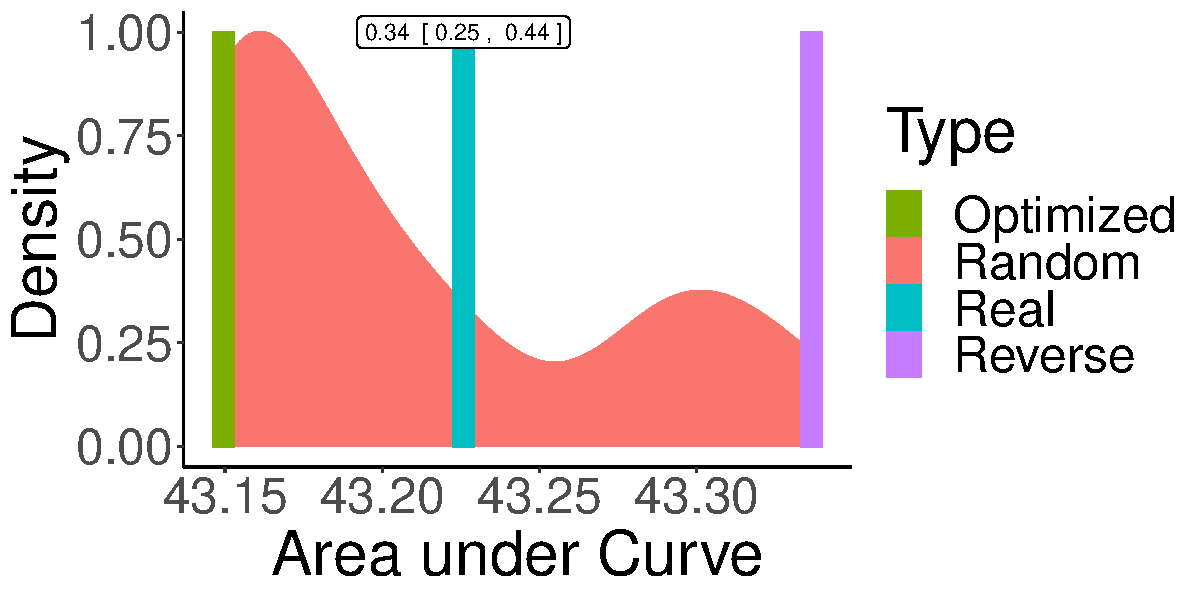
\includegraphics[width=0.3\textwidth]{figures/finnish_verbs/suffixes-byMorphemes-auc-hist-heldout-Coarse-FineSurprisal-optimized.pdf}
        &
    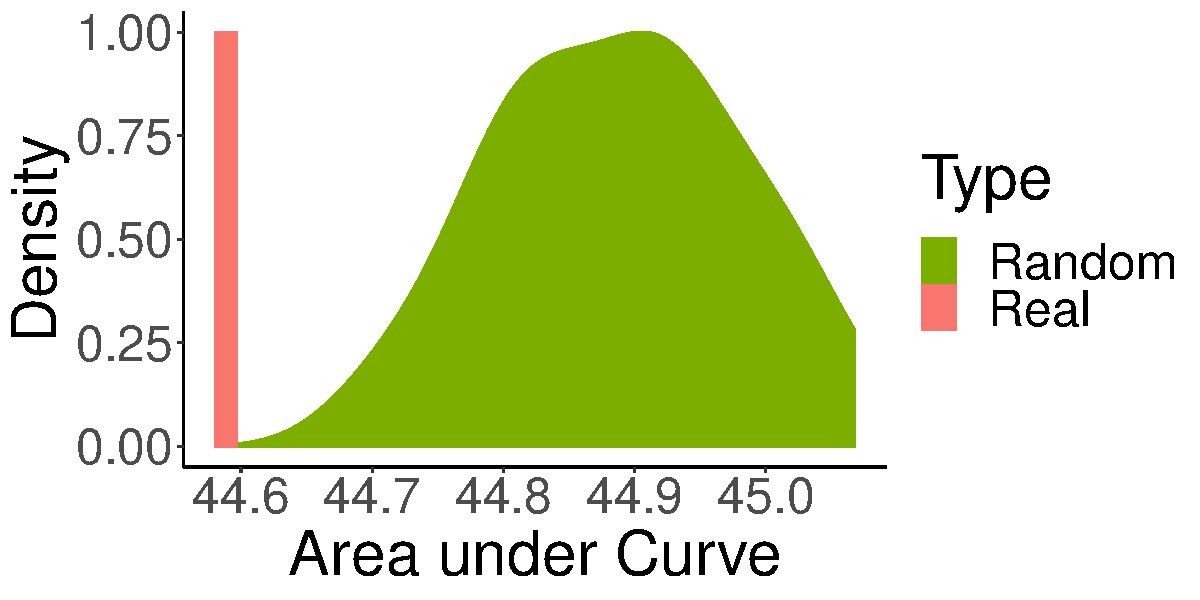
\includegraphics[width=0.3\textwidth]{figures/turkish_verbs/suffixes-byMorphemes-auc-hist-heldout-Coarse-FineSurprisal-optimized.pdf}
    &
    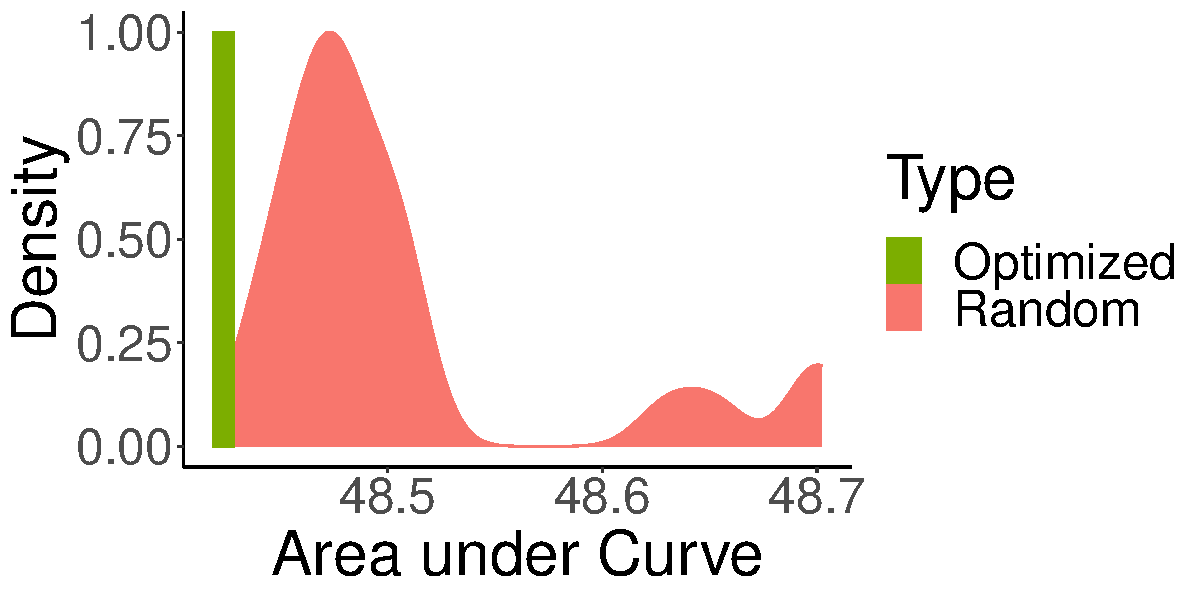
\includegraphics[width=0.3\textwidth]{figures/hungarian_verbs/suffixes-byMorphemes-auc-hist-heldout-Coarse-FineSurprisal-optimized.pdf}
    \\
    \textsc{Korean} & \textsc{Japanese} & \textsc{Sesotho Prefixes} \\
    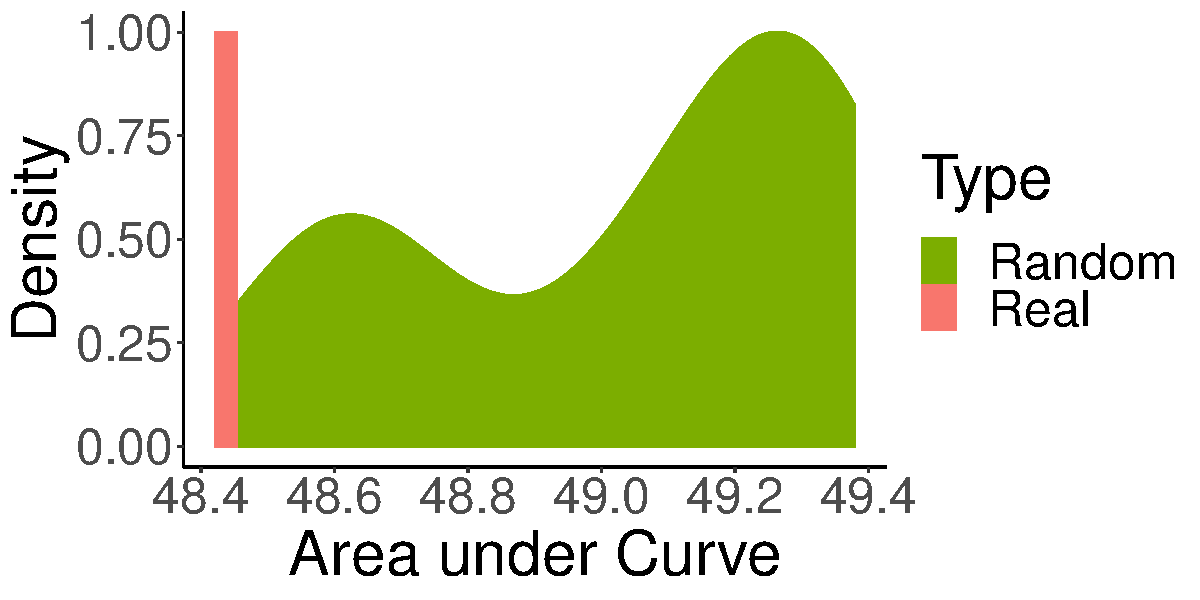
\includegraphics[width=0.3\textwidth]{figures/korean/suffixes-byMorphemes-auc-hist-heldout-Coarse-FineSurprisal-optimized.pdf}
    &
        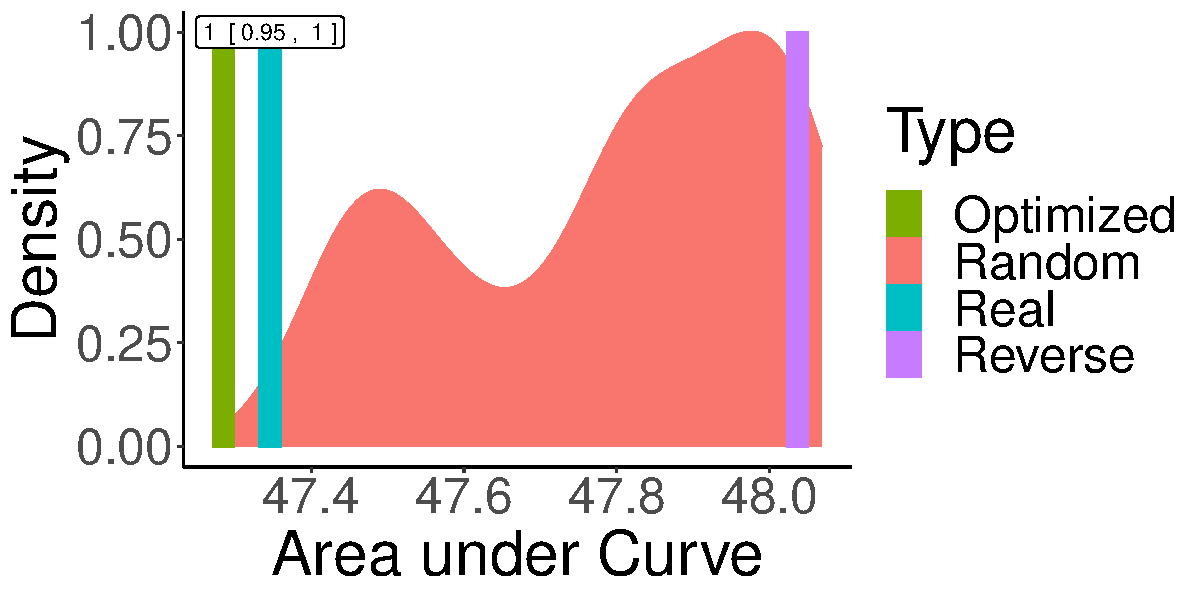
\includegraphics[width=0.3\textwidth]{figures/japanese/suffixes-byMorphemes-auc-hist-heldout-Coarse-FineSurprisal-optimized.pdf}
        &
            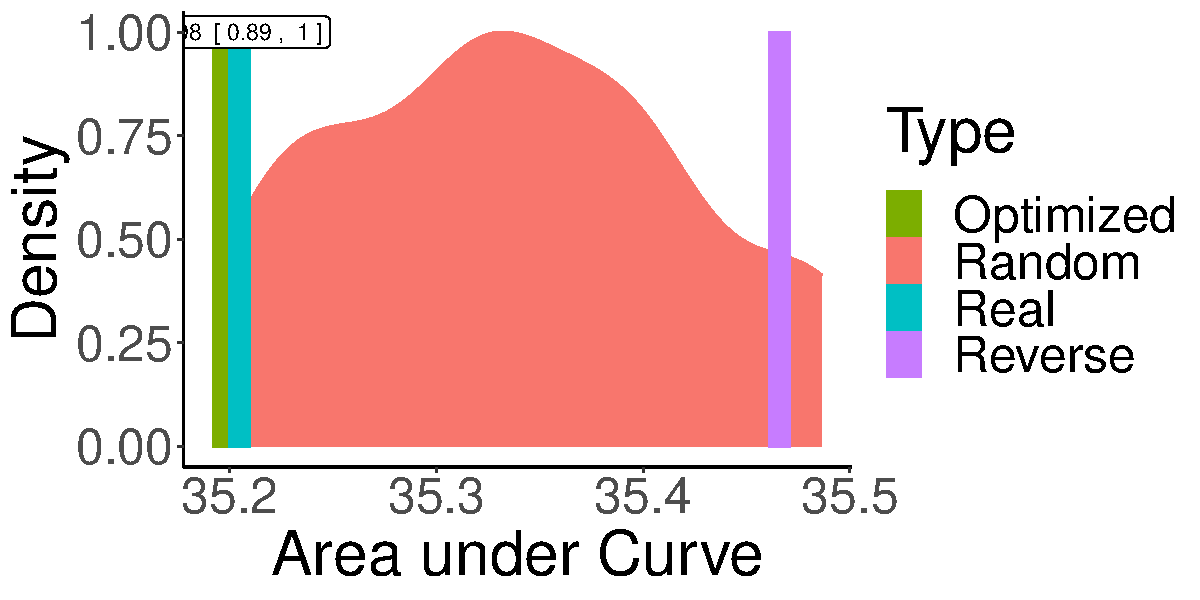
\includegraphics[width=0.3\textwidth]{figures/sesotho_prefixes/suffixes-byMorphemes-auc-hist-heldout-Coarse-FineSurprisal-optimized.pdf}
            \\
            \textsc{Sesotho Suffixes} \\
            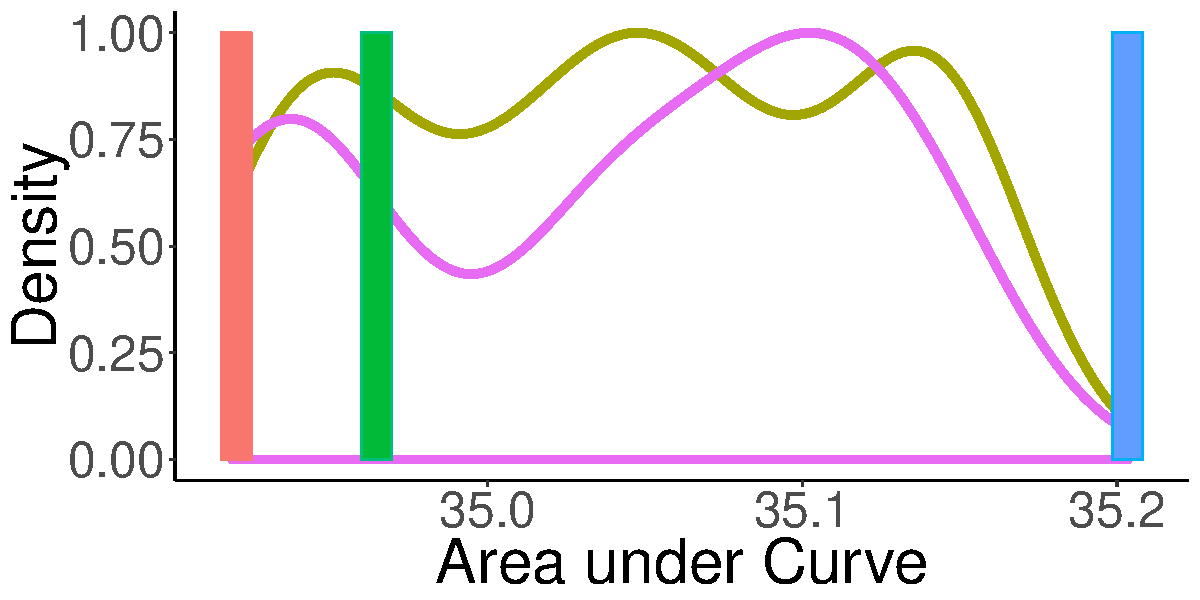
\includegraphics[width=0.3\textwidth]{figures/sesotho_suffixes/suffixes-byMorphemes-auc-hist-heldout-Coarse-FineSurprisal-optimized.pdf}
    \end{tabular}

    
    \caption{AUC Histograms for Verb Affixes.}
    \label{fig:auc_verbs}
\end{figure}


\begin{figure}
\begin{tabular}{ccc}
\textsc{Finnish} & \textsc{Turkish} & \textsc{Hungarian} \\
    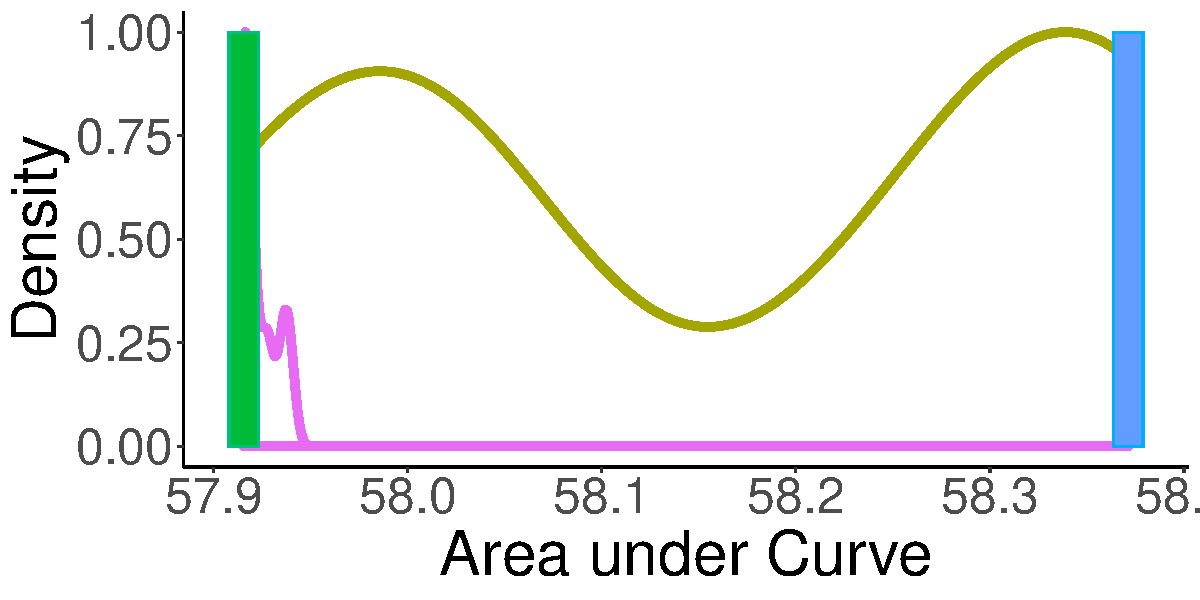
\includegraphics[width=0.3\textwidth]{figures/finnish_nouns/suffixes-byMorphemes-auc-hist-heldout-Coarse-FineSurprisal-optimized.pdf}
    &
    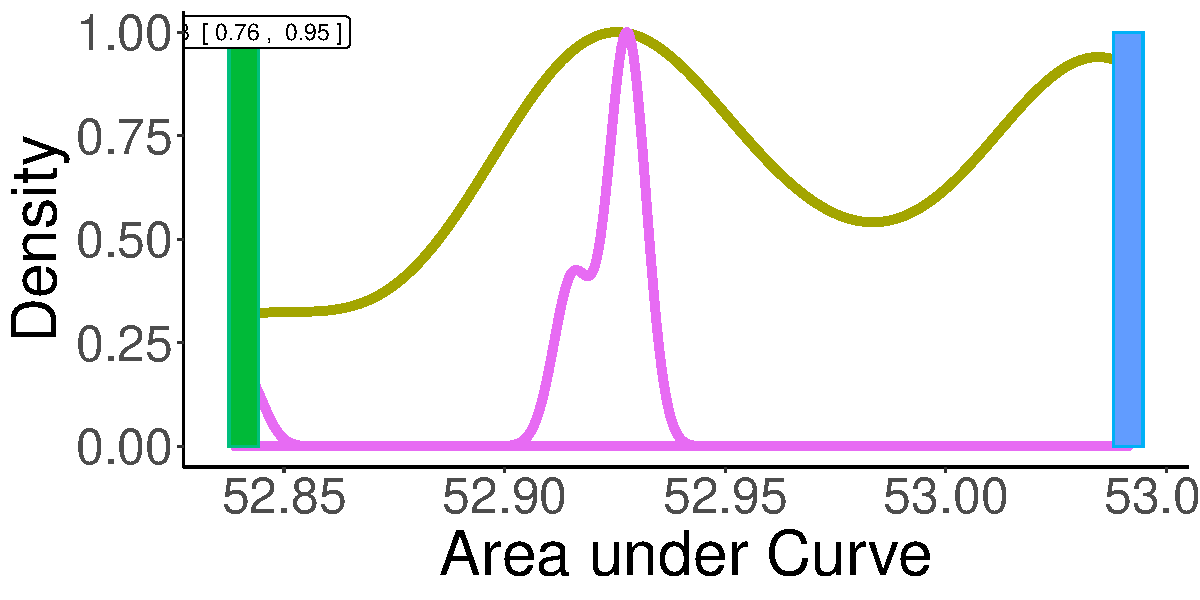
\includegraphics[width=0.3\textwidth]{figures/turkish_nouns/suffixes-byMorphemes-auc-hist-heldout-Coarse-FineSurprisal-optimized.pdf}
    &
    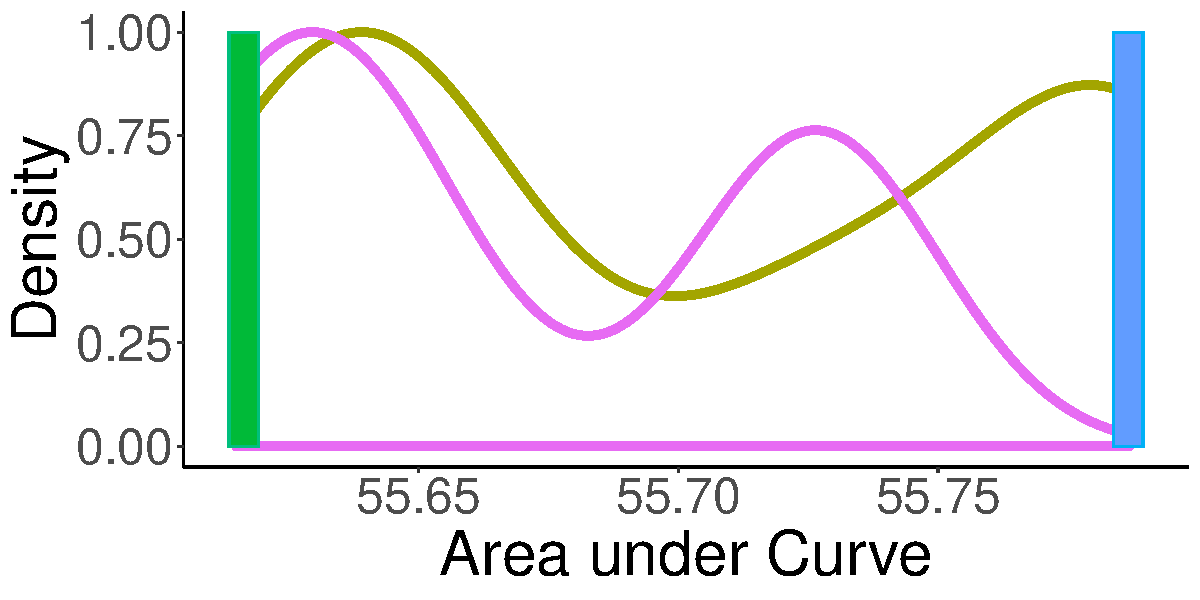
\includegraphics[width=0.3\textwidth]{figures/hungarian_nouns/suffixes-byMorphemes-auc-hist-heldout-Coarse-FineSurprisal-optimized.pdf}
    \end{tabular}
    \caption{Noun Suffixes}
    \label{fig:auc_nouns}
\end{figure}

\begin{table}[]
    \centering
    \begin{tabular}{l|l|ll|lllllllll}
    &     &    \multicolumn{2}{c|}{Pairs} & \multicolumn{2}{c|}{Full} & \multicolumn{2}{c}{Full (Types)} \\
     &   &     Optim. & Baseline & Optim. & Baseline & Optim. & Baseline \\ \hline
 & finnish nouns & 1.0 (0.0) & 0.42 (0.31) & 1.0 (0.0) & 0.37 (0.32) & 1.0 (0.0) & 0.38 (0.29) \\
 & turkish nouns & 1.0 (0.0) & 0.56 (0.36) & 1.0 (0.0) & 0.5 (0.37) & 1.0 (0.0) & 0.5 (0.36) \\
 & hungarian nouns & 1.0 (0.0) & 0.48 (0.22) & 1.0 (0.0) & 0.33 (0.27) & 1.0 (0.0) & 0.33 (0.27) \\
 \hline
 & finnish verbs & 0.4 (0.3) & 0.4 (0.37) & 0.38 (0.31) & 0.39 (0.38) & 0.36 (0.32) & 0.38 (0.37) \\
 & hungarian verbs & 0.95 (0.09) & 0.52 (0.37) & 0.95 (0.0) & 0.5 (0.4) & 0.94 (0.0) & 0.5 (0.39) \\
 & turkish verbs & 0.96 (0.09) & 0.46 (0.14) & 0.95 (0.0) & 0.37 (0.15) & 0.93 (0.07) & 0.36 (0.14) \\
 & korean & 0.97 (0.1) & 0.56 (0.33) & 0.97 (0.0) & 0.53 (0.33) & 0.95 (0.0) & 0.53 (0.36) \\
 & japanese & 0.94 (0.08) & 0.48 (0.24) & 0.93 (0.0) & 0.39 (0.24) & 0.9 (0.1) & 0.39 (0.24) \\
 & sesotho prefixes & 0.99 (0.0) & 0.5 (0.48) & 0.99 (0.0) & 0.5 (0.48) & 0.98 (0.0) & 0.51 (0.46) \\
 & sesotho suffixes & 0.62 (0.0) & 0.48 (0.2) & 0.54 (0.0) & 0.45 (0.19) & 0.52 (0.0) & 0.44 (0.19) \\
    \end{tabular}
    \caption{Accuracies in predicting morpheme ordering. `Optim.' indicates grammars optimized for AUC, `'Baseline' indicates randomly constructed weights.
    In each cell, we provide the mean and the stgandard deviation over orderings. `Pairs' indicates the fraction of pairs of morphemes occurring together in the same word that are ordered correctly. `Full' indicates the fraction of verb forms in the corpus that are ordered fully correctly. `Full (Types)' counts forms that occur multiple times only once, it thus down-weights the role of frequent forms.}
    \label{tab:optimized_acc}
\end{table}



\begin{figure}[]
\begin{tabular}{cccccccc}
\textsc{Turkish} & \textsc{Hungarian} & \textsc{Finnish} \\
\begin{minipage}{.3\textwidth}
    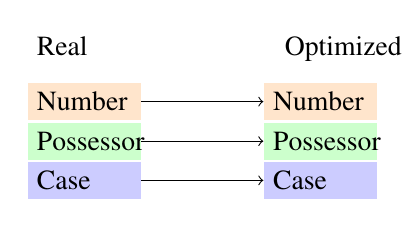
\begin{tikzpicture}[%
% common options for blocks:
block/.style = {draw, fill=blue!30, align=center, anchor=west,
            minimum height=0.65cm, inner sep=0},
% common options for the circles:
ball/.style = {circle, draw, align=center, anchor=north, inner sep=0}]
\node[rectangle,text width=1.2cm,anchor=base] (A0) at (1,-0.3) {Real};
\node[rectangle,text width=0.9cm,anchor=base] (B0) at (4,-0.3) {Optimized};
\node[rectangle,text width=1.2cm,anchor=base, fill=orange!20] (A1) at (1,-1.0) {Number};
\node[rectangle,text width=1.2cm,anchor=base, fill=green!20] (A2) at (1,-1.5) {Possessor};
\node[rectangle,text width=1.2cm,anchor=base, fill=blue!20] (A3) at (1,-2.0) {Case};
\node[rectangle,text width=1.2cm,anchor=base, fill=orange!20] (B1) at (4,-1.0) {Number};
\node[rectangle,text width=1.2cm,anchor=base, fill=green!20] (B2) at (4,-1.5) {Possessor};
\node[rectangle,text width=1.2cm,anchor=base, fill=blue!20] (B3) at (4,-2.0) {Case};
\draw[->] (A1.east) to (B1.west);
\draw[->] (A2.east) to (B2.west);
\draw[->] (A3.east) to (B3.west);
\end{tikzpicture}

    \end{minipage}
  &
  \begin{minipage}{.3\textwidth}
    \begin{tikzpicture}[%
% common options for blocks:
block/.style = {draw, fill=blue!30, align=center, anchor=west,
            minimum height=0.65cm, inner sep=0},
% common options for the circles:
ball/.style = {circle, draw, align=center, anchor=north, inner sep=0}]
\node[rectangle,text width=1.2cm,anchor=base] (A0) at (1,-0.3) {Real};
\node[rectangle,text width=0.9cm,anchor=base] (B0) at (4,-0.3) {Optimized};
\node[rectangle,text width=1.2cm,anchor=base] (A1) at (1,-1.0) {Number};
\node[rectangle,text width=1.2cm,anchor=base] (A2) at (1,-1.5) {Psor_person};
\node[rectangle,text width=1.2cm,anchor=base] (A3) at (1,-2.0) {Psor_number};
\node[rectangle,text width=1.2cm,anchor=base] (A4) at (1,-2.5) {Case};
\node[rectangle,text width=1.2cm,anchor=base] (B1) at (4,-1.0) {Number};
\node[rectangle,text width=1.2cm,anchor=base] (B2) at (4,-1.5) {Psor_person};
\node[rectangle,text width=1.2cm,anchor=base] (B3) at (4,-2.0) {Psor_number};
\node[rectangle,text width=1.2cm,anchor=base] (B4) at (4,-2.5) {Case};
\draw[->] (A1.east) to (B1.west);
\draw[->] (A2.east) to (B2.west);
\draw[->] (A3.east) to (B3.west);
\draw[->] (A4.east) to (B4.west);
\end{tikzpicture}

    \end{minipage}
  &
  \begin{minipage}{.3\textwidth}
    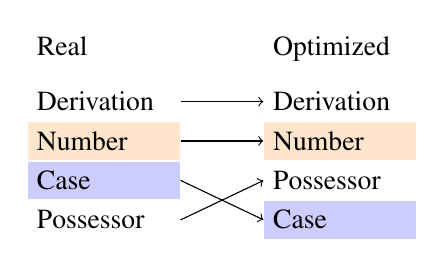
\begin{tikzpicture}[%
% common options for blocks:
block/.style = {draw, fill=blue!30, align=center, anchor=west,
            minimum height=0.65cm, inner sep=0},
% common options for the circles:
ball/.style = {circle, draw, align=center, anchor=north, inner sep=0}]
\node[rectangle,text width=1.7cm,anchor=base] (A0) at (1,-0.3) {Real};
\node[rectangle,text width=1.7cm,anchor=base] (B0) at (4,-0.3) {Optimized};
\node[rectangle,text width=1.7cm,anchor=base] (A1) at (1,-1.0) {Derivation};
\node[rectangle,text width=1.7cm,anchor=base, fill=orange!20] (A2) at (1,-1.5) {Number};
\node[rectangle,text width=1.7cm,anchor=base, fill=blue!20] (A3) at (1,-2.0) {Case};
\node[rectangle,text width=1.7cm,anchor=base] (A4) at (1,-2.5) {Possessor};
\node[rectangle,text width=1.7cm,anchor=base] (B1) at (4,-1.0) {Derivation};
\node[rectangle,text width=1.7cm,anchor=base, fill=orange!20] (B2) at (4,-1.5) {Number};
\node[rectangle,text width=1.7cm,anchor=base] (B3) at (4,-2.0) {Possessor};
\node[rectangle,text width=1.7cm,anchor=base, fill=blue!20] (B4) at (4,-2.5) {Case};
\draw[->] (A1.east) to (B1.west);
\draw[->] (A2.east) to (B2.west);
\draw[->] (A3.east) to (B4.west);
\draw[->] (A4.east) to (B3.west);
\end{tikzpicture}

  \end{minipage}
  \end{tabular}
  
    \caption{Real and optimized ordering (nouns)}
    \label{fig:real_and_optimized_nouns}
\end{figure}


\begin{figure}[]

\begin{tabular}{cccccccc}
\textsc{Turkish} & \textsc{Hungarian} & \textsc{Finnish} \\
\begin{minipage}{.3\textwidth}
    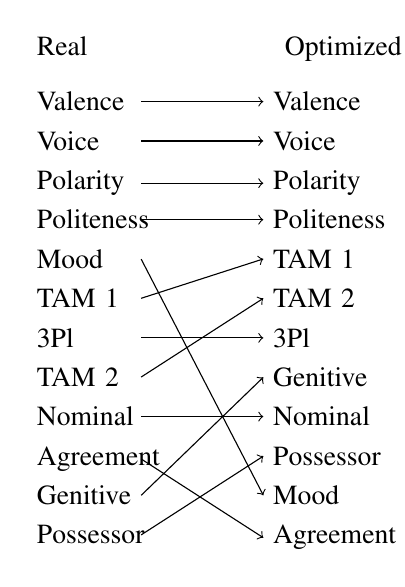
\begin{tikzpicture}[%
% common options for blocks:
block/.style = {draw, fill=blue!30, align=center, anchor=west,
            minimum height=0.65cm, inner sep=0},
% common options for the circles:
ball/.style = {circle, draw, align=center, anchor=north, inner sep=0}]
\node[rectangle,text width=1.2cm,anchor=base] (A0) at (1,-0.3) {Real};
\node[rectangle,text width=0.9cm,anchor=base] (B0) at (4,-0.3) {Optimized};
\node[rectangle,text width=1.2cm,anchor=base] (A1) at (1,-1.0) {Valence};
\node[rectangle,text width=1.2cm,anchor=base] (A2) at (1,-1.5) {Voice};
\node[rectangle,text width=1.2cm,anchor=base] (A3) at (1,-2.0) {Polarity};
\node[rectangle,text width=1.2cm,anchor=base] (A4) at (1,-2.5) {Politeness};
\node[rectangle,text width=1.2cm,anchor=base] (A5) at (1,-3.0) {Mood};
\node[rectangle,text width=1.2cm,anchor=base] (A6) at (1,-3.5) {TAM 1};
\node[rectangle,text width=1.2cm,anchor=base] (A7) at (1,-4.0) {3Pl};
\node[rectangle,text width=1.2cm,anchor=base] (A8) at (1,-4.5) {TAM 2};
\node[rectangle,text width=1.2cm,anchor=base] (A9) at (1,-5.0) {Nominal};
\node[rectangle,text width=1.2cm,anchor=base] (A10) at (1,-5.5) {Agreement};
\node[rectangle,text width=1.2cm,anchor=base] (A11) at (1,-6.0) {Genitive};
\node[rectangle,text width=1.2cm,anchor=base] (A12) at (1,-6.5) {Possessor};
\node[rectangle,text width=1.2cm,anchor=base] (B1) at (4,-1.0) {Valence};
\node[rectangle,text width=1.2cm,anchor=base] (B2) at (4,-1.5) {Voice};
\node[rectangle,text width=1.2cm,anchor=base] (B3) at (4,-2.0) {Polarity};
\node[rectangle,text width=1.2cm,anchor=base] (B4) at (4,-2.5) {Politeness};
\node[rectangle,text width=1.2cm,anchor=base] (B5) at (4,-3.0) {TAM 1};
\node[rectangle,text width=1.2cm,anchor=base] (B6) at (4,-3.5) {TAM 2};
\node[rectangle,text width=1.2cm,anchor=base] (B7) at (4,-4.0) {3Pl};
\node[rectangle,text width=1.2cm,anchor=base] (B8) at (4,-4.5) {Genitive};
\node[rectangle,text width=1.2cm,anchor=base] (B9) at (4,-5.0) {Nominal};
\node[rectangle,text width=1.2cm,anchor=base] (B10) at (4,-5.5) {Possessor};
\node[rectangle,text width=1.2cm,anchor=base] (B11) at (4,-6.0) {Mood};
\node[rectangle,text width=1.2cm,anchor=base] (B12) at (4,-6.5) {Agreement};
\draw[->] (A1.east) to (B1.west);
\draw[->] (A2.east) to (B2.west);
\draw[->] (A3.east) to (B3.west);
\draw[->] (A4.east) to (B4.west);
\draw[->] (A5.east) to (B11.west);
\draw[->] (A6.east) to (B5.west);
\draw[->] (A7.east) to (B7.west);
\draw[->] (A8.east) to (B6.west);
\draw[->] (A9.east) to (B9.west);
\draw[->] (A10.east) to (B12.west);
\draw[->] (A11.east) to (B8.west);
\draw[->] (A12.east) to (B10.west);
\end{tikzpicture}

  \end{minipage}
  &
  \begin{minipage}{.3\textwidth}
    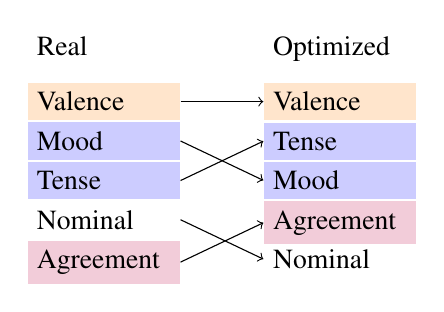
\begin{tikzpicture}[%
% common options for blocks:
block/.style = {draw, fill=blue!30, align=center, anchor=west,
            minimum height=0.65cm, inner sep=0},
% common options for the circles:
ball/.style = {circle, draw, align=center, anchor=north, inner sep=0}]
\node[rectangle,text width=1.7cm,anchor=base] (A0) at (1,-0.3) {Real};
\node[rectangle,text width=1.7cm,anchor=base] (B0) at (4,-0.3) {Optimized};
\node[rectangle,text width=1.7cm,anchor=base, fill=orange!20] (A1) at (1,-1.0) {Valence};
\node[rectangle,text width=1.7cm,anchor=base, fill=blue!20] (A2) at (1,-1.5) {Mood};
\node[rectangle,text width=1.7cm,anchor=base, fill=blue!20] (A3) at (1,-2.0) {Tense};
\node[rectangle,text width=1.7cm,anchor=base] (A4) at (1,-2.5) {Nominal};
\node[rectangle,text width=1.7cm,anchor=base, fill=purple!20] (A5) at (1,-3.0) {Agreement};
\node[rectangle,text width=1.7cm,anchor=base, fill=orange!20] (B1) at (4,-1.0) {Valence};
\node[rectangle,text width=1.7cm,anchor=base, fill=blue!20] (B2) at (4,-1.5) {Tense};
\node[rectangle,text width=1.7cm,anchor=base, fill=blue!20] (B3) at (4,-2.0) {Mood};
\node[rectangle,text width=1.7cm,anchor=base, fill=purple!20] (B4) at (4,-2.5) {Agreement};
\node[rectangle,text width=1.7cm,anchor=base] (B5) at (4,-3.0) {Nominal};
\draw[->] (A1.east) to (B1.west);
\draw[->] (A2.east) to (B3.west);
\draw[->] (A3.east) to (B2.west);
\draw[->] (A4.east) to (B5.west);
\draw[->] (A5.east) to (B4.west);
\end{tikzpicture}

  \end{minipage}
  &
    \begin{minipage}{.3\textwidth}
    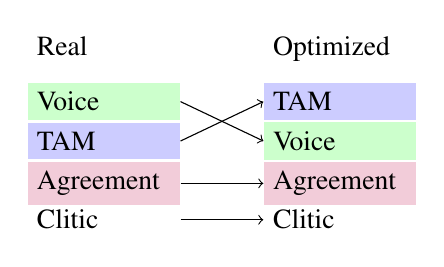
\begin{tikzpicture}[%
% common options for blocks:
block/.style = {draw, fill=blue!30, align=center, anchor=west,
            minimum height=0.65cm, inner sep=0},
% common options for the circles:
ball/.style = {circle, draw, align=center, anchor=north, inner sep=0}]
\node[rectangle,text width=1.7cm,anchor=base] (A0) at (1,-0.3) {Real};
\node[rectangle,text width=1.7cm,anchor=base] (B0) at (4,-0.3) {Optimized};
\node[rectangle,text width=1.7cm,anchor=base, fill=green!20] (A1) at (1,-1.0) {Voice};
\node[rectangle,text width=1.7cm,anchor=base, fill=blue!20] (A2) at (1,-1.5) {TAM};
\node[rectangle,text width=1.7cm,anchor=base, fill=purple!20] (A3) at (1,-2.0) {Agreement};
\node[rectangle,text width=1.7cm,anchor=base] (A4) at (1,-2.5) {Clitic};
\node[rectangle,text width=1.7cm,anchor=base, fill=blue!20] (B1) at (4,-1.0) {TAM};
\node[rectangle,text width=1.7cm,anchor=base, fill=green!20] (B2) at (4,-1.5) {Voice};
\node[rectangle,text width=1.7cm,anchor=base, fill=purple!20] (B3) at (4,-2.0) {Agreement};
\node[rectangle,text width=1.7cm,anchor=base] (B4) at (4,-2.5) {Clitic};
\draw[->] (A1.east) to (B2.west);
\draw[->] (A2.east) to (B1.west);
\draw[->] (A3.east) to (B3.west);
\draw[->] (A4.east) to (B4.west);
\end{tikzpicture}

  \end{minipage}
  \\
  \textsc{Korean}  & \textsc{Japanese} & \textsc{Sesotho Prefixes} \\
      \begin{minipage}{.3\textwidth}
    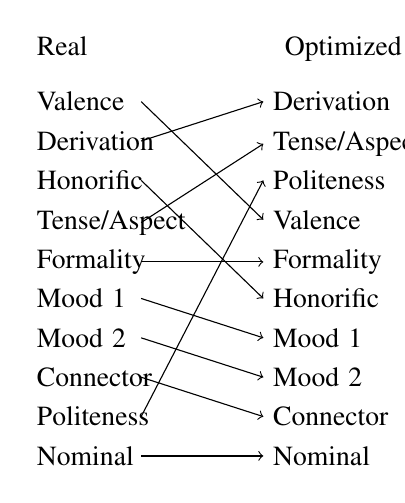
\begin{tikzpicture}[%
% common options for blocks:
block/.style = {draw, fill=blue!30, align=center, anchor=west,
            minimum height=0.65cm, inner sep=0},
% common options for the circles:
ball/.style = {circle, draw, align=center, anchor=north, inner sep=0}]
\node[rectangle,text width=1.2cm,anchor=base] (A0) at (1,-0.3) {Real};
\node[rectangle,text width=0.9cm,anchor=base] (B0) at (4,-0.3) {Optimized};
\node[rectangle,text width=1.2cm,anchor=base] (A1) at (1,-1.0) {Valence};
\node[rectangle,text width=1.2cm,anchor=base] (A2) at (1,-1.5) {Derivation};
\node[rectangle,text width=1.2cm,anchor=base] (A3) at (1,-2.0) {Honorific};
\node[rectangle,text width=1.2cm,anchor=base] (A4) at (1,-2.5) {Tense/Aspect};
\node[rectangle,text width=1.2cm,anchor=base] (A5) at (1,-3.0) {Formality};
\node[rectangle,text width=1.2cm,anchor=base] (A6) at (1,-3.5) {Mood 1};
\node[rectangle,text width=1.2cm,anchor=base] (A7) at (1,-4.0) {Mood 2};
\node[rectangle,text width=1.2cm,anchor=base] (A8) at (1,-4.5) {Connector};
\node[rectangle,text width=1.2cm,anchor=base] (A9) at (1,-5.0) {Politeness};
\node[rectangle,text width=1.2cm,anchor=base] (A10) at (1,-5.5) {Nominal};
\node[rectangle,text width=1.2cm,anchor=base] (B1) at (4,-1.0) {Derivation};
\node[rectangle,text width=1.2cm,anchor=base] (B2) at (4,-1.5) {Tense/Aspect};
\node[rectangle,text width=1.2cm,anchor=base] (B3) at (4,-2.0) {Politeness};
\node[rectangle,text width=1.2cm,anchor=base] (B4) at (4,-2.5) {Valence};
\node[rectangle,text width=1.2cm,anchor=base] (B5) at (4,-3.0) {Formality};
\node[rectangle,text width=1.2cm,anchor=base] (B6) at (4,-3.5) {Honorific};
\node[rectangle,text width=1.2cm,anchor=base] (B7) at (4,-4.0) {Mood 1};
\node[rectangle,text width=1.2cm,anchor=base] (B8) at (4,-4.5) {Mood 2};
\node[rectangle,text width=1.2cm,anchor=base] (B9) at (4,-5.0) {Connector};
\node[rectangle,text width=1.2cm,anchor=base] (B10) at (4,-5.5) {Nominal};
\draw[->] (A1.east) to (B4.west);
\draw[->] (A2.east) to (B1.west);
\draw[->] (A3.east) to (B6.west);
\draw[->] (A4.east) to (B2.west);
\draw[->] (A5.east) to (B5.west);
\draw[->] (A6.east) to (B7.west);
\draw[->] (A7.east) to (B8.west);
\draw[->] (A8.east) to (B9.west);
\draw[->] (A9.east) to (B3.west);
\draw[->] (A10.east) to (B10.west);
\end{tikzpicture}

  \end{minipage}
  &
  \begin{minipage}{.3\textwidth}
    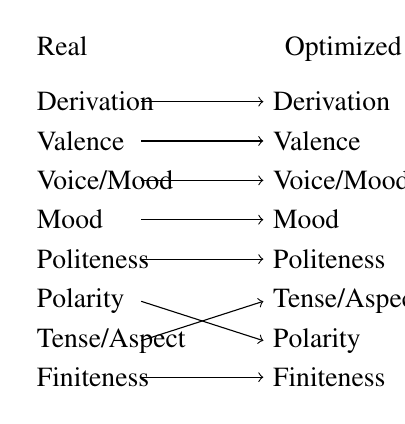
\begin{tikzpicture}[%
% common options for blocks:
block/.style = {draw, fill=blue!30, align=center, anchor=west,
            minimum height=0.65cm, inner sep=0},
% common options for the circles:
ball/.style = {circle, draw, align=center, anchor=north, inner sep=0}]
\node[rectangle,text width=1.2cm,anchor=base] (A0) at (1,-0.3) {Real};
\node[rectangle,text width=0.9cm,anchor=base] (B0) at (4,-0.3) {Optimized};
\node[rectangle,text width=1.2cm,anchor=base] (A1) at (1,-1.0) {Derivation};
\node[rectangle,text width=1.2cm,anchor=base] (A2) at (1,-1.5) {Valence};
\node[rectangle,text width=1.2cm,anchor=base] (A3) at (1,-2.0) {Voice/Mood};
\node[rectangle,text width=1.2cm,anchor=base] (A4) at (1,-2.5) {Mood};
\node[rectangle,text width=1.2cm,anchor=base] (A5) at (1,-3.0) {Politeness};
\node[rectangle,text width=1.2cm,anchor=base] (A6) at (1,-3.5) {Polarity};
\node[rectangle,text width=1.2cm,anchor=base] (A7) at (1,-4.0) {Tense/Aspect};
\node[rectangle,text width=1.2cm,anchor=base] (A8) at (1,-4.5) {Finiteness};
\node[rectangle,text width=1.2cm,anchor=base] (B1) at (4,-1.0) {Derivation};
\node[rectangle,text width=1.2cm,anchor=base] (B2) at (4,-1.5) {Valence};
\node[rectangle,text width=1.2cm,anchor=base] (B3) at (4,-2.0) {Voice/Mood};
\node[rectangle,text width=1.2cm,anchor=base] (B4) at (4,-2.5) {Mood};
\node[rectangle,text width=1.2cm,anchor=base] (B5) at (4,-3.0) {Politeness};
\node[rectangle,text width=1.2cm,anchor=base] (B6) at (4,-3.5) {Tense/Aspect};
\node[rectangle,text width=1.2cm,anchor=base] (B7) at (4,-4.0) {Polarity};
\node[rectangle,text width=1.2cm,anchor=base] (B8) at (4,-4.5) {Finiteness};
\draw[->] (A1.east) to (B1.west);
\draw[->] (A2.east) to (B2.west);
\draw[->] (A3.east) to (B3.west);
\draw[->] (A4.east) to (B4.west);
\draw[->] (A5.east) to (B5.west);
\draw[->] (A6.east) to (B7.west);
\draw[->] (A7.east) to (B6.west);
\draw[->] (A8.east) to (B8.west);
\end{tikzpicture}

  \end{minipage}
  &
  \begin{minipage}{.3\textwidth}
    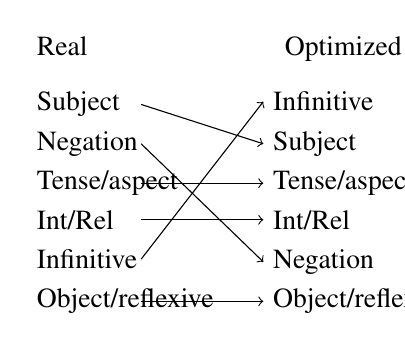
\begin{tikzpicture}[%
% common options for blocks:
block/.style = {draw, fill=blue!30, align=center, anchor=west,
            minimum height=0.65cm, inner sep=0},
% common options for the circles:
ball/.style = {circle, draw, align=center, anchor=north, inner sep=0}]
\node[rectangle,text width=1.2cm,anchor=base] (A0) at (1,-0.3) {Real};
\node[rectangle,text width=0.9cm,anchor=base] (B0) at (4,-0.3) {Optimized};
\node[rectangle,text width=1.2cm,anchor=base] (A1) at (1,-1.0) {Subject};
\node[rectangle,text width=1.2cm,anchor=base] (A2) at (1,-1.5) {Negation};
\node[rectangle,text width=1.2cm,anchor=base] (A3) at (1,-2.0) {Tense/aspect};
\node[rectangle,text width=1.2cm,anchor=base] (A4) at (1,-2.5) {Int/Rel};
\node[rectangle,text width=1.2cm,anchor=base] (A5) at (1,-3.0) {Infinitive};
\node[rectangle,text width=1.2cm,anchor=base] (A6) at (1,-3.5) {Object/reflexive};
\node[rectangle,text width=1.2cm,anchor=base] (B1) at (4,-1.0) {Infinitive};
\node[rectangle,text width=1.2cm,anchor=base] (B2) at (4,-1.5) {Subject};
\node[rectangle,text width=1.2cm,anchor=base] (B3) at (4,-2.0) {Tense/aspect};
\node[rectangle,text width=1.2cm,anchor=base] (B4) at (4,-2.5) {Int/Rel};
\node[rectangle,text width=1.2cm,anchor=base] (B5) at (4,-3.0) {Negation};
\node[rectangle,text width=1.2cm,anchor=base] (B6) at (4,-3.5) {Object/reflexive};
\draw[->] (A1.east) to (B2.west);
\draw[->] (A2.east) to (B5.west);
\draw[->] (A3.east) to (B3.west);
\draw[->] (A4.east) to (B4.west);
\draw[->] (A5.east) to (B1.west);
\draw[->] (A6.east) to (B6.west);
\end{tikzpicture}

  \end{minipage} \\
  \textsc{Sesotho Suffixes} \\
  \begin{minipage}{.3\textwidth}
    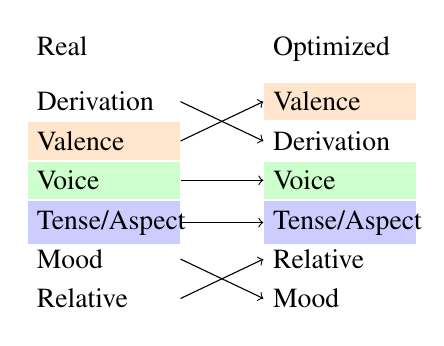
\begin{tikzpicture}[%
% common options for blocks:
block/.style = {draw, fill=blue!30, align=center, anchor=west,
            minimum height=0.65cm, inner sep=0},
% common options for the circles:
ball/.style = {circle, draw, align=center, anchor=north, inner sep=0}]
\node[rectangle,text width=1.7cm,anchor=base] (A0) at (1,-0.3) {Real};
\node[rectangle,text width=1.7cm,anchor=base] (B0) at (4,-0.3) {Optimized};
\node[rectangle,text width=1.7cm,anchor=base] (A1) at (1,-1.0) {Derivation};
\node[rectangle,text width=1.7cm,anchor=base, fill=orange!20] (A2) at (1,-1.5) {Valence};
\node[rectangle,text width=1.7cm,anchor=base, fill=green!20] (A3) at (1,-2.0) {Voice};
\node[rectangle,text width=1.7cm,anchor=base, fill=blue!20] (A4) at (1,-2.5) {Tense/Aspect};
\node[rectangle,text width=1.7cm,anchor=base] (A5) at (1,-3.0) {Mood};
\node[rectangle,text width=1.7cm,anchor=base] (A6) at (1,-3.5) {Relative};
\node[rectangle,text width=1.7cm,anchor=base, fill=orange!20] (B1) at (4,-1.0) {Valence};
\node[rectangle,text width=1.7cm,anchor=base] (B2) at (4,-1.5) {Derivation};
\node[rectangle,text width=1.7cm,anchor=base, fill=green!20] (B3) at (4,-2.0) {Voice};
\node[rectangle,text width=1.7cm,anchor=base, fill=blue!20] (B4) at (4,-2.5) {Tense/Aspect};
\node[rectangle,text width=1.7cm,anchor=base] (B5) at (4,-3.0) {Relative};
\node[rectangle,text width=1.7cm,anchor=base] (B6) at (4,-3.5) {Mood};
\draw[->] (A1.east) to (B2.west);
\draw[->] (A2.east) to (B1.west);
\draw[->] (A3.east) to (B3.west);
\draw[->] (A4.east) to (B4.west);
\draw[->] (A5.east) to (B6.west);
\draw[->] (A6.east) to (B5.west);
\end{tikzpicture}

  \end{minipage}
  \end{tabular}
  
  
    \caption{Real and optimized ordering (verbs)}
    \label{fig:real_and_optimized_verbs}
\end{figure}



\begin{figure}
\begin{tabular}{ccccccc}
\textsc{Finnish} & \textsc{Hungarian} & \textsc{Turkish} \\
\begin{minipage}{.3\textwidth}
    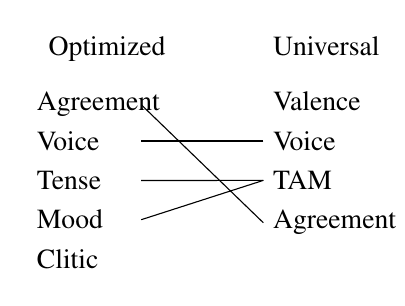
\begin{tikzpicture}[%
% common options for blocks:
block/.style = {draw, fill=blue!30, align=center, anchor=west,
            minimum height=0.65cm, inner sep=0},
% common options for the circles:
ball/.style = {circle, draw, align=center, anchor=north, inner sep=0}]
\node[rectangle,text width=1.2cm,anchor=base] (A0) at (4,-0.3) {Universal};
\node[rectangle,text width=0.9cm,anchor=base] (B0) at (1,-0.3) {Optimized};
\node[rectangle,text width=1.2cm,anchor=base] (A1) at (4,-1.0) {Valence};
\node[rectangle,text width=1.2cm,anchor=base] (A2) at (4,-1.5) {Voice};
\node[rectangle,text width=1.2cm,anchor=base] (A3) at (4,-2.0) {TAM};
\node[rectangle,text width=1.2cm,anchor=base] (A4) at (4,-2.5) {Agreement};
\node[rectangle,text width=1.2cm,anchor=base] (B1) at (1,-1.0) {Agreement};
\node[rectangle,text width=1.2cm,anchor=base] (B2) at (1,-1.5) {Voice};
\node[rectangle,text width=1.2cm,anchor=base] (B3) at (1,-2.0) {Tense};
\node[rectangle,text width=1.2cm,anchor=base] (B4) at (1,-2.5) {Mood};
\node[rectangle,text width=1.2cm,anchor=base] (B5) at (1,-3.0) {Clitic};
\draw[-] (A4.west) to (B1.east);
\draw[-] (A2.west) to (B2.east);
\draw[-] (A3.west) to (B3.east);
\draw[-] (A3.west) to (B4.east);
\end{tikzpicture}

    \end{minipage}
    &
    \begin{minipage}{.3\textwidth}
    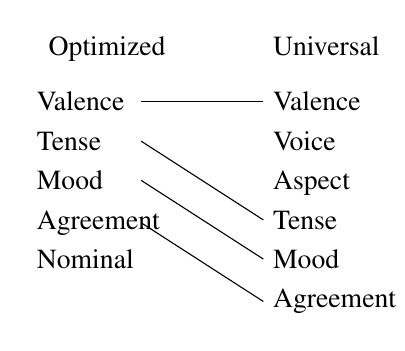
\begin{tikzpicture}[%
% common options for blocks:
block/.style = {draw, fill=blue!30, align=center, anchor=west,
            minimum height=0.65cm, inner sep=0},
% common options for the circles:
ball/.style = {circle, draw, align=center, anchor=north, inner sep=0}]
\node[rectangle,text width=1.2cm,anchor=base] (A0) at (4,-0.3) {Universal};
\node[rectangle,text width=0.9cm,anchor=base] (B0) at (1,-0.3) {Optimized};
\node[rectangle,text width=1.2cm,anchor=base] (A1) at (4,-1.0) {Valence};
\node[rectangle,text width=1.2cm,anchor=base] (A2) at (4,-1.5) {Voice};
\node[rectangle,text width=1.2cm,anchor=base] (A3) at (4,-2.0) {Aspect};
\node[rectangle,text width=1.2cm,anchor=base] (A4) at (4,-2.5) {Tense};
\node[rectangle,text width=1.2cm,anchor=base] (A5) at (4,-3.0) {Mood};
\node[rectangle,text width=1.2cm,anchor=base] (A6) at (4,-3.5) {Agreement};
\node[rectangle,text width=1.2cm,anchor=base] (B1) at (1,-1.0) {Valence};
\node[rectangle,text width=1.2cm,anchor=base] (B2) at (1,-1.5) {Tense};
\node[rectangle,text width=1.2cm,anchor=base] (B3) at (1,-2.0) {Mood};
\node[rectangle,text width=1.2cm,anchor=base] (B4) at (1,-2.5) {Agreement};
\node[rectangle,text width=1.2cm,anchor=base] (B5) at (1,-3.0) {Nominal};
\draw[-] (A1.west) to (B1.east);
\draw[-] (A4.west) to (B2.east);
\draw[-] (A5.west) to (B3.east);
\draw[-] (A6.west) to (B4.east);
\end{tikzpicture}

    \end{minipage}
        &
    \begin{minipage}{.3\textwidth}
    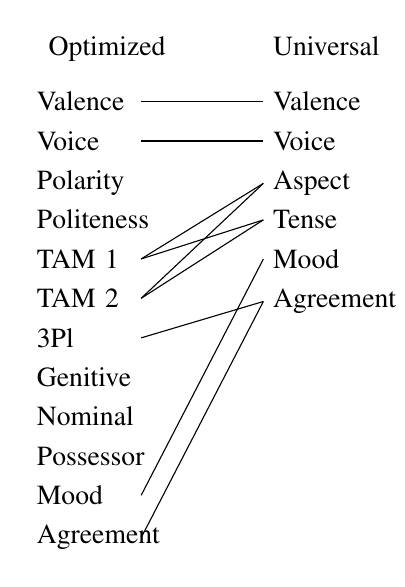
\begin{tikzpicture}[%
% common options for blocks:
block/.style = {draw, fill=blue!30, align=center, anchor=west,
            minimum height=0.65cm, inner sep=0},
% common options for the circles:
ball/.style = {circle, draw, align=center, anchor=north, inner sep=0}]
\node[rectangle,text width=1.2cm,anchor=base] (A0) at (4,-0.3) {Universal};
\node[rectangle,text width=0.9cm,anchor=base] (B0) at (1,-0.3) {Optimized};
\node[rectangle,text width=1.2cm,anchor=base] (A1) at (4,-1.0) {Valence};
\node[rectangle,text width=1.2cm,anchor=base] (A2) at (4,-1.5) {Voice};
\node[rectangle,text width=1.2cm,anchor=base] (A3) at (4,-2.0) {Aspect};
\node[rectangle,text width=1.2cm,anchor=base] (A4) at (4,-2.5) {Tense};
\node[rectangle,text width=1.2cm,anchor=base] (A5) at (4,-3.0) {Mood};
\node[rectangle,text width=1.2cm,anchor=base] (A6) at (4,-3.5) {Agreement};
\node[rectangle,text width=1.2cm,anchor=base] (B1) at (1,-1.0) {Valence};
\node[rectangle,text width=1.2cm,anchor=base] (B2) at (1,-1.5) {Voice};
\node[rectangle,text width=1.2cm,anchor=base] (B3) at (1,-2.0) {Polarity};
\node[rectangle,text width=1.2cm,anchor=base] (B4) at (1,-2.5) {Politeness};
\node[rectangle,text width=1.2cm,anchor=base] (B5) at (1,-3.0) {TAM 1};
\node[rectangle,text width=1.2cm,anchor=base] (B6) at (1,-3.5) {TAM 2};
\node[rectangle,text width=1.2cm,anchor=base] (B7) at (1,-4.0) {3Pl};
\node[rectangle,text width=1.2cm,anchor=base] (B8) at (1,-4.5) {Genitive};
\node[rectangle,text width=1.2cm,anchor=base] (B9) at (1,-5.0) {Nominal};
\node[rectangle,text width=1.2cm,anchor=base] (B10) at (1,-5.5) {Possessor};
\node[rectangle,text width=1.2cm,anchor=base] (B11) at (1,-6.0) {Mood};
\node[rectangle,text width=1.2cm,anchor=base] (B12) at (1,-6.5) {Agreement};
\draw[-] (A1.west) to (B1.east);
\draw[-] (A2.west) to (B2.east);
\draw[-] (A3.west) to (B5.east);
\draw[-] (A4.west) to (B5.east);
\draw[-] (A3.west) to (B6.east);
\draw[-] (A4.west) to (B6.east);
\draw[-] (A6.west) to (B7.east);
\draw[-] (A5.west) to (B11.east);
\draw[-] (A6.west) to (B12.east);
\end{tikzpicture}

    \end{minipage} 
    \\
    \textsc{Korean} & \textsc{Japanese} & \textsc{Sesotho Prefixes} \\
        \begin{minipage}{.3\textwidth}
    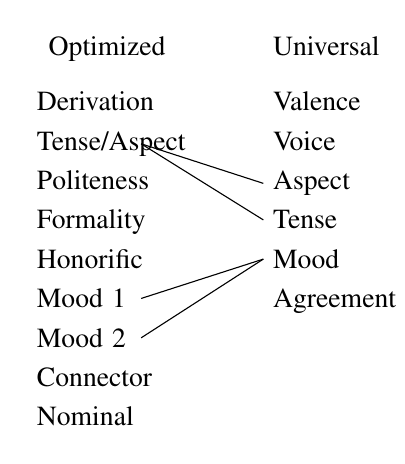
\begin{tikzpicture}[%
% common options for blocks:
block/.style = {draw, fill=blue!30, align=center, anchor=west,
            minimum height=0.65cm, inner sep=0},
% common options for the circles:
ball/.style = {circle, draw, align=center, anchor=north, inner sep=0}]
\node[rectangle,text width=1.2cm,anchor=base] (A0) at (4,-0.3) {Universal};
\node[rectangle,text width=0.9cm,anchor=base] (B0) at (1,-0.3) {Optimized};
\node[rectangle,text width=1.2cm,anchor=base] (A1) at (4,-1.0) {Valence};
\node[rectangle,text width=1.2cm,anchor=base] (A2) at (4,-1.5) {Voice};
\node[rectangle,text width=1.2cm,anchor=base] (A3) at (4,-2.0) {Aspect};
\node[rectangle,text width=1.2cm,anchor=base] (A4) at (4,-2.5) {Tense};
\node[rectangle,text width=1.2cm,anchor=base] (A5) at (4,-3.0) {Mood};
\node[rectangle,text width=1.2cm,anchor=base] (A6) at (4,-3.5) {Agreement};
\node[rectangle,text width=1.2cm,anchor=base] (B1) at (1,-1.0) {Derivation};
\node[rectangle,text width=1.2cm,anchor=base] (B2) at (1,-1.5) {Tense/Aspect};
\node[rectangle,text width=1.2cm,anchor=base] (B3) at (1,-2.0) {Politeness};
\node[rectangle,text width=1.2cm,anchor=base] (B4) at (1,-2.5) {Formality};
\node[rectangle,text width=1.2cm,anchor=base] (B5) at (1,-3.0) {Honorific};
\node[rectangle,text width=1.2cm,anchor=base] (B6) at (1,-3.5) {Mood 1};
\node[rectangle,text width=1.2cm,anchor=base] (B7) at (1,-4.0) {Mood 2};
\node[rectangle,text width=1.2cm,anchor=base] (B8) at (1,-4.5) {Connector};
\node[rectangle,text width=1.2cm,anchor=base] (B9) at (1,-5.0) {Nominal};
\draw[-] (A3.west) to (B2.east);
\draw[-] (A4.west) to (B2.east);
\draw[-] (A5.west) to (B6.east);
\draw[-] (A5.west) to (B7.east);
\end{tikzpicture}

    \end{minipage}
    &
    \begin{minipage}{.3\textwidth}
    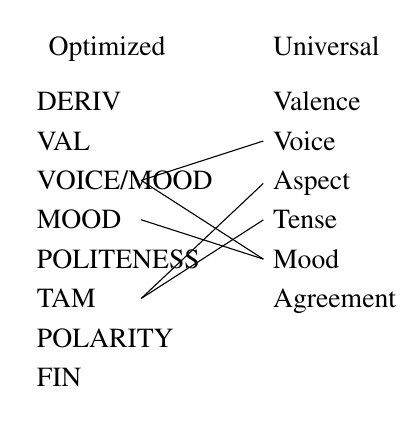
\begin{tikzpicture}[%
% common options for blocks:
block/.style = {draw, fill=blue!30, align=center, anchor=west,
            minimum height=0.65cm, inner sep=0},
% common options for the circles:
ball/.style = {circle, draw, align=center, anchor=north, inner sep=0}]
\node[rectangle,text width=1.2cm,anchor=base] (A0) at (4,-0.3) {Universal};
\node[rectangle,text width=0.9cm,anchor=base] (B0) at (1,-0.3) {Optimized};
\node[rectangle,text width=1.2cm,anchor=base] (A1) at (4,-1.0) {Valence};
\node[rectangle,text width=1.2cm,anchor=base] (A2) at (4,-1.5) {Voice};
\node[rectangle,text width=1.2cm,anchor=base] (A3) at (4,-2.0) {Aspect};
\node[rectangle,text width=1.2cm,anchor=base] (A4) at (4,-2.5) {Tense};
\node[rectangle,text width=1.2cm,anchor=base] (A5) at (4,-3.0) {Mood};
\node[rectangle,text width=1.2cm,anchor=base] (A6) at (4,-3.5) {Agreement};
\node[rectangle,text width=1.2cm,anchor=base] (B1) at (1,-1.0) {DERIV};
\node[rectangle,text width=1.2cm,anchor=base] (B2) at (1,-1.5) {VAL};
\node[rectangle,text width=1.2cm,anchor=base] (B3) at (1,-2.0) {VOICE/MOOD};
\node[rectangle,text width=1.2cm,anchor=base] (B4) at (1,-2.5) {MOOD};
\node[rectangle,text width=1.2cm,anchor=base] (B5) at (1,-3.0) {POLITENESS};
\node[rectangle,text width=1.2cm,anchor=base] (B6) at (1,-3.5) {TAM};
\node[rectangle,text width=1.2cm,anchor=base] (B7) at (1,-4.0) {POLARITY};
\node[rectangle,text width=1.2cm,anchor=base] (B8) at (1,-4.5) {FIN};
\draw[-] (A2.west) to (B3.east);
\draw[-] (A5.west) to (B3.east);
\draw[-] (A5.west) to (B4.east);
\draw[-] (A3.west) to (B6.east);
\draw[-] (A4.west) to (B6.east);
\end{tikzpicture}

    \end{minipage}
        &
    \begin{minipage}{.3\textwidth}
    \begin{tikzpicture}[%
% common options for blocks:
block/.style = {draw, fill=blue!30, align=center, anchor=west,
            minimum height=0.65cm, inner sep=0},
% common options for the circles:
ball/.style = {circle, draw, align=center, anchor=north, inner sep=0}]
\node[rectangle,text width=1.2cm,anchor=base] (A0) at (4,-0.3) {Universal};
\node[rectangle,text width=0.9cm,anchor=base] (B0) at (1,-0.3) {Optimized};
\node[rectangle,text width=1.2cm,anchor=base] (A1) at (4,-1.0) {Valence};
\node[rectangle,text width=1.2cm,anchor=base] (A2) at (4,-1.5) {Voice};
\node[rectangle,text width=1.2cm,anchor=base] (A3) at (4,-2.0) {Aspect};
\node[rectangle,text width=1.2cm,anchor=base] (A4) at (4,-2.5) {Tense};
\node[rectangle,text width=1.2cm,anchor=base] (A5) at (4,-3.0) {Mood};
\node[rectangle,text width=1.2cm,anchor=base] (A6) at (4,-3.5) {Agreement};
\node[rectangle,text width=1.2cm,anchor=base] (B1) at (1,-1.0) {Other_6};
\node[rectangle,text width=1.2cm,anchor=base] (B2) at (1,-1.5) {Other_2a};
\node[rectangle,text width=1.2cm,anchor=base] (B3) at (1,-2.0) {Infinitive};
\node[rectangle,text width=1.2cm,anchor=base] (B4) at (1,-2.5) {Other_ij};
\node[rectangle,text width=1.2cm,anchor=base] (B5) at (1,-3.0) {Other_wo};
\node[rectangle,text width=1.2cm,anchor=base] (B6) at (1,-3.5) {Other_di};
\node[rectangle,text width=1.2cm,anchor=base] (B7) at (1,-4.0) {Other_copula};
\node[rectangle,text width=1.2cm,anchor=base] (B8) at (1,-4.5) {Other_1s};
\node[rectangle,text width=1.2cm,anchor=base] (B9) at (1,-5.0) {Other_lo};
\node[rectangle,text width=1.2cm,anchor=base] (B10) at (1,-5.5) {Subject};
\node[rectangle,text width=1.2cm,anchor=base] (B11) at (1,-6.0) {Other_f^};
\node[rectangle,text width=1.2cm,anchor=base] (B12) at (1,-6.5) {Other_2};
\node[rectangle,text width=1.2cm,anchor=base] (B13) at (1,-7.0) {Tense/aspect};
\node[rectangle,text width=1.2cm,anchor=base] (B14) at (1,-7.5) {Int/Rel};
\node[rectangle,text width=1.2cm,anchor=base] (B15) at (1,-8.0) {Other_av};
\node[rectangle,text width=1.2cm,anchor=base] (B16) at (1,-8.5) {Negation};
\node[rectangle,text width=1.2cm,anchor=base] (B17) at (1,-9.0) {Other_9};
\node[rectangle,text width=1.2cm,anchor=base] (B18) at (1,-9.5) {Other_3};
\node[rectangle,text width=1.2cm,anchor=base] (B19) at (1,-10.0) {Other_17};
\node[rectangle,text width=1.2cm,anchor=base] (B20) at (1,-10.5) {Other_10};
\node[rectangle,text width=1.2cm,anchor=base] (B21) at (1,-11.0) {Other_7};
\node[rectangle,text width=1.2cm,anchor=base] (B22) at (1,-11.5) {Other_pr};
\node[rectangle,text width=1.2cm,anchor=base] (B23) at (1,-12.0) {Object/reflexive};
\draw[-] (A6.west) to (B10.east);
\draw[-] (A3.west) to (B13.east);
\draw[-] (A4.west) to (B13.east);
\draw[-] (A1.west) to (B23.east);
\end{tikzpicture}

    \end{minipage}
    \\
    \textsc{Sesotho Suffixes} \\
        \begin{minipage}{.3\textwidth}
    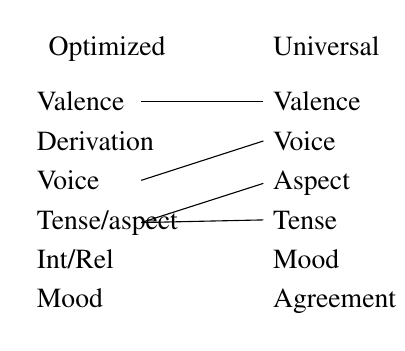
\begin{tikzpicture}[%
% common options for blocks:
block/.style = {draw, fill=blue!30, align=center, anchor=west,
            minimum height=0.65cm, inner sep=0},
% common options for the circles:
ball/.style = {circle, draw, align=center, anchor=north, inner sep=0}]
\node[rectangle,text width=1.2cm,anchor=base] (A0) at (4,-0.3) {Universal};
\node[rectangle,text width=0.9cm,anchor=base] (B0) at (1,-0.3) {Optimized};
\node[rectangle,text width=1.2cm,anchor=base] (A1) at (4,-1.0) {Valence};
\node[rectangle,text width=1.2cm,anchor=base] (A2) at (4,-1.5) {Voice};
\node[rectangle,text width=1.2cm,anchor=base] (A3) at (4,-2.0) {Aspect};
\node[rectangle,text width=1.2cm,anchor=base] (A4) at (4,-2.5) {Tense};
\node[rectangle,text width=1.2cm,anchor=base] (A5) at (4,-3.0) {Mood};
\node[rectangle,text width=1.2cm,anchor=base] (A6) at (4,-3.5) {Agreement};
\node[rectangle,text width=1.2cm,anchor=base] (B1) at (1,-1.0) {Valence};
\node[rectangle,text width=1.2cm,anchor=base] (B2) at (1,-1.5) {Derivation};
\node[rectangle,text width=1.2cm,anchor=base] (B3) at (1,-2.0) {Voice};
\node[rectangle,text width=1.2cm,anchor=base] (B4) at (1,-2.5) {Tense/aspect};
\node[rectangle,text width=1.2cm,anchor=base] (B5) at (1,-3.0) {Int/Rel};
\node[rectangle,text width=1.2cm,anchor=base] (B6) at (1,-3.5) {Mood};
\draw[-] (A1.west) to (B1.east);
\draw[-] (A2.west) to (B3.east);
\draw[-] (A3.west) to (B4.east);
\draw[-] (A4.west) to (B4.east);
\end{tikzpicture}

    \end{minipage}
\end{tabular}
    \caption{Comparing optimized orders with the universal order described by \citep{bybee-morphology-1985}.  Note that, for Sesotho prefixes, inversion of order relative to the universal order is expected, as the universal order indicates distance from the root, not absolute position.}
    \label{fig:optimized_and_universal_orders}
\end{figure}


\section{Discussion}

We have examined morpheme order in nouns and verbs in six languages, testing the recently propiosed Efficient Tradeoff Hypothesis \citep{hahn2020modeling} as an explanatory account of morpheme ordering.
We compared actual morpheme orderings to other possible orderings and to orderings optimized for efficiency of the memory-surprisal tradeoff.
In most cases, we found that the real ordering provided more efficient tradeoffs than most alternative orderings.
More importantly, we found that the real orderings match the optimal orderings in many respects.
Ordering forms found in a corpus according according to real or optimized orderings yields the same orders in XXX of cases.
In some cases, particularly for noun inflection, match between real and optimized orderings is perfect.
Beyond language-specific ordering patterns, optimization recovers several previously-documented language universals of morpheme order.

\subsection{Relation to previous accounts}

%\subsubsection{Semantic Scope; Syntactic Structure; Historical Development}

In this section, we discuss the linguistic literature on morpheme ordering.

\paragraph{Levels of Linguistic Description}

Morpheme ordering has been described from the perspective 

Besides the explanation of broad typological tendencies, which we are interested in here, the linguistic literature has also debated at which level of linguistic representation morpheme ordering should be described, proposing accounts located at different levels such as the syntax-phonology interface \citep{baker1985the} and an autonomous layer of morphological description \citep{hyman2003suffix}.
%TODO also template vs scope vs...
We do not see the memory--surprisal tradeoff as competing with or contradicting these studies.
Rather, it specifies tendencies for ordering that could be implemented at different levels of linguistic description.


%\paragraph{Revelance and Proximity}
As mentioned in section \becky{cite S2}, Bybee proposes a concept of \textit{semantic relevance}, which is the degree to which one morpheme affects the semantic content of the other \becky{cite bybee}. She hypothesizes that morphemes that are more highly relevant to each other should be closer to each other, and therefore proposes a universal ordering of verbal inflectional morphemes. For example, attaching a causative marker to a root meaning "to die" produces a verb form meaning "to kill." Since the causative greatly changes the semantic content of the original root, the causative is highly relevant to the root. 

\becky{Format Korean example of juk-da ``to die" and juk-i-da ``to kill"}

Bybee did not provide a way to computationally measure semantic relevance. However, our optimized orders of Turkish and Hungarian \becky{Are there other languages?} perfectly match Bybee's proposed universal verbal inflection order \becky{need a figure comparing optimized order to Bybee's order}. This suggests that high mutual information generally correlates with semantic relevance. 


A related family of explanations holds that those affixes are closest to the root that are most relevant to the root \citep{bybee-morphology-1985}.
Other explanations suggest that morphemes are ordered based on (TODO CITE).
The most straightforwardly related account is that of Bybee (1985) Semantic relevance
CARP template in Bantu
Explanations for the orders

talk about Relevance and Mutual Information


%\paragraph{Morphemes as Fossilized Words}
It has long been observed that the order of morphemes often parallels the order of independent words of corresponding meanings \citep{givon1971historical,venneman1973explanation,baker1985the}.
It has been argued that the order of morphemes reflects the order of formerly independent elements that have been fossilized into bound morphemes \citet{givon1971historical,venneman1973explanation}.
As the memory-surprisal tradeoff is optimized by word order, this is compatible with our results:
To the extent that morpheme order does reflect fossilized word order, morpheme order should continue to reflect optimization for the tradeoff.

On the other hand, \citet{bybee-morphology-1985} points out that there are historically documented cases where morpheme ordering has been restructured in ways that do not reflect former independent words, but respect the universal tendencies proposed by her (see also \citet{mithun2000the, haspelmath1993the, mithun1995affixation}; \citet[Section 15]{rice2000morpheme}).
As a theory of order at multiple levels, the memory-surprisal tradeoff predicts these ordering patterns independent of the historical path leading to the morphemes found in a given language.



syntax-phonology interface \citep{baker1985the} 
For instance, 
\cite{baker1985the} proposed the Mirror Principle, which -- informally -- states that the order of elements (morphemes) in morphology reflects the order of elements (words) in syntax.

Also noted scope: \citep{baker1988incorporation,foley1984functional,chierchia1990meaning,valin1992a}


%This can be related to the scope-based explanation to the extent that syntactic structure and word order reflect scope.
% INTERESTING reference: http://www.jzeller.de/pdf/CARP.pdf

%\paragraph{Semantic Scope}


A related account is in terms of semantic scope \cite{rice2000morpheme}.
The relative ordering of valence and voice is a good example for the scope-based explanation.
Valence affixes change the number of arguments, and passive (voice) promotes one argument to the subject position.
This can affect an argument introduced by a voice marker.
The following example from Turkish illustrates this (\cite{schaaik2020turkish}, section 30.8.2):

\begin{tabular}{ccccccc}
don-dur-ul & freeze-caus-pass & be frozen \\
don-dur & freeze-caus & to freeze (something) \\
don & freeze& to freeze \\
\end{tabular}

In contrast, adding the passive marker to the root \textit{don} is illicit as the root verb is intransitive.

Description in terms of scope faces limitations when order is different from semantic scope.
Hyman  (2003:  249) proposed the CARP template to describe suffix order in Bantu languages (such as Sesotho), a templatic order for valence and voice morphemes that can be different from scope order.

\paragraph{Templates}
CARP template


\cite{muysken1981quechua}

\cite{mccarthy2008generalized} phonology

\cite{hyman2003suffix}

\cite{kanu2009suffix} morphotactics, not semantic scope



See SI Apenndix Section X for simulations arguing that scope and mutual information may correlate.

%\subsection{Relevance; Proximity; Iconicity}

%The relation  between mutual information and relevance






\subsection{Beyond Agglutionation}

Our study focused on agglutinatioon, where a word carries multiple clearly separated morphemes with distinct functions.
There are other types of morphological processes that deserve study.

While we have focused on the relative distance from the root, we have not touched on the question of why a morpheme is realized as a prefix or a suffix in a given language.
There are well-known correlations between suffixing or prefixing preference and word order \citep{greenberg1963universals}.

- infixation

Vowel change, productive in many languages and fossilized in English (swim $\rightarrow$ swam).

non-concatenative morphology (in Arabic, k-t-b `to write' forms katab- `wrote'. -aktub `write/be writing', -kutib- `was written').

\subsection{Limitations}

- genre of data: written. but Sesotho is spoken (child-directed)


- limitations of computational estimation of the memory-surprisal tradeoff

As the set of all moprphological forms of a language is typically finite (CITE), we believe that these limitations play a smaller role in morpheme order, compared to word order.


A further limitation relates to the selection of languages.
The six languages considered in this study are spoken in Eurasia and Africa, not representing Australia and America.
Among the languages, Hungarian and Finnish are genetically related (X millenia).
There is also some evidence for genetic relations beyond these (Japanese, Korean, Turkish), but such relations would have to be quite ancient (x millenia).
The morphemes found in these languages as considered here are generally not cognate.
Thus, the commonalities in languages found cannot be traced to inherited orderings of morphemes inherited from a common ancestor.
Furthermore, we note that the optimality of different orderings crucially depend not on the morphemes themselves (which might be inherited), but on the frequencies of different forms (e.g., of sinulars and plurals).



\section{Conclusion}

We have tested the recently proposed Memory-Surprisal Tradeoff as a predictor of morpheme order with data from verbs and nouns across six languages.
We found that attested morpheme orders provide more efficient tradeoffs than most other possible orderings and that many properties of observed orderings are recovered by optimizing for tradeoff efficiency.
With the exception of verb inflection in Finnish and Sesotho, we found that optimized orderings agree with the attested orderings in more than 90\% of forms found in corpora.
Optimization also successfully predicts several universals of morpheme ordering, both for nouns and verbs.


\bibliography{literature}
\bibliographystyle{natbib}
\appendix

\section{Appendix}


\subsection{Estimating Memory--Surprisal Tradeoffs}


\subsection{Korean Verb Suffixes}

Korean verb morphology is very complex, and there is no generally agreed-upon description in terms of morphemes and slots.
We extracted suffixes based on the annotation found in the Kaist corpus and the linguistic literature on Korean \citep{yeon2010korean}.
The Kaist corpus provides segmentation into morphemes; we postprocessed it in two ways:
First, we made it more fine-grained by splitting morphemes that are merged in the annotation, and, second, we abstracted away consistently from allomorphy.
For instance, the Kaist corpus separately labels the segments \korean{ㅂ니다} \textit{-mnida} (as in \korean{합니다} \textit{hamnida} `does') and \korean{습니다} \textit{-seumnida} (as in \korean{했습니다} \textit{hatseumnida} `did').
These two segments actually are allomorphs, conditioned by the preceding material.
Furthermore, they can both be segmented into the formal marker \korean{ㅂ/습} (\textit{-p/-seup}, we label this underlying morpheme ``\textsc{p}$_5$'', see below for this notation), and the mood markers \korean{니} (\textit{-ni}, our \textsc{ni}$_6$) and \korean{다} (\textit{-da}, our \textsc{da}$_7$).
We therefore transform both segments into the abstract morpheme sequence \textsc{p}$_5$-\textsc{ni}$_6$-\textsc{da}$_7$ (see below for this notation).
We then partitioned the resulting morphemes into slots that make it possible to consistently describe the ordering of almost all forms encountered in the corpus.


With this procedure, we identified the nine slots described below. We show morphemes occurring at least 50 times in slots 2-8 in Figure~\ref{tab:korean-frequent-morphemes}.
We do not provide the list of conjunctive and nominalizing suffixes since these are very numerous.

Additional morphemes that occur less than X times are placed into an UNKNOWN slots, this affects X \% of morpheme occurrences in the dataset.
We indicate morphemes by a small-caps representation of a stylized phonological representation (such as \textsc{p} for -\korean{ㅂ/습}  -\textit{p/seup}),\footnote{These transcriptions are purely conventional, we do not intend these to correspond to a theory of how underlying phonological forms are realized as surface phone strings.} with a subscript indicating their slot (such as \textsc{p}$_5$-\textsc{ni}$_6$-\textsc{da}$_7$).

\begin{enumerate}
    \item Root
    %. The root may include a valency suffix, which is not separated frem the root in the dataset. We did not attempt to separate v
    \item Derivation: The two derivational suffixes are \textit{ha} (\citep[4.1.2]{yeon2010korean}) and the predicative \textit{i}, whose function is similar to that of a copula \citep[4.1.4]{yeon2010korean}.
    
    \item Honorific \textsc{si}$_3$ \citep[4.3.2, 4.4.1]{yeon2010korean}
    \item Tense/Aspect suffixes include -\textsc{ess}$_4$ for past \citep[4.5.1.1]{yeon2010korean}, -\textsc{essess}$_4$ for remote past \citep[4.5.1.2]{yeon2010korean}, -\textsc{get}$_4$ for future \citep[4.5.2.1]{yeon2010korean}
    \item Formality \textsc{p}$_5$ (allomorphs include -\textit{p}-, -\textit{m}-, -\textit{seum}-,  \citep[4.3.2]{yeon2010korean})
    \item We partition Mood suffixes into two slots, as these can be combined. Frequent elements of the Mood I slot are -\textsc{n}$_6$-, -\textsc{ni}$_6$- \citep[4.3.2]{yeon2010korean}.
    
    \item Frequent elements of the Mood II slot are declarative -\textsc{da}$_7$- \citep[4.3.2]{yeon2010korean}, command -\textsc{ra}-, interrogative -\textsc{ka}-, the suffix  -\textsc{ji} \citep[4.2.2-3]{yeon2010korean}, and informal -\textsc{eo}$_7$- (informal).
    
    \item Polite -yo
    \item Conjunctive endings
    
    -go
    
    -seo
    
    and others
    
\end{enumerate}

TODO 

- Yeon 4.4.2.2 kkeo object honorific % 꺼

%\ex.\ag. oa di rek a \\
%\textsc{subject.agreement} \textsc{object.agreement} buy \textsc{indicative} \\
%`(he) is buying (it)'  \citep{demuth1992acquisition} \label{ex:oadireka}
%\bg. o pheh el a \\
%\textsc{subject.agreement} cook \textsc{applicative} \textsc{indicative} \\
%`(he) cooks (food) for (him)'  \citep{demuth1992acquisition}
%\label{ex:ophehela}


%Examples:
%\begin{tabular}{llllllllll}
%1    & 3 & 4     & 5   & 6  & 7 & 8 \\
%bara & sy & eots & eum & ni & da  & &  `wished'\\
%wish & Honorific & Past & Formal & Indicative & Indicative \\
%bara& & gess &  & &  eo & yo  &  `will wish' \\
%wish  & &  Assertive && & informal & polite \\
%\end{tabular}


%Frequent morphemes:
\begin{table}
\resizebox{1.2\textwidth}{!}{
\begin{tabular}{llllllllll}
Slot & Morphs & Short & Freq. & Description & Citation \\ \hline\hline
Derivation & \korean{하} & HA$_2$ &	 68 & & \citep[4.1.2]{yeon2010korean}\\
& i & I$_2$ &	 3947 && \citep[4.1.4]{yeon2010korean} \\ \hline
Honorific & si 	& \textsc{si}$_3$ & 99 & &\citep[4.3.2, 4.4.1]{yeon2010korean}\\\hline
Tense/Asp. & \korean{었었} 	& ESSESS$_4$ &  56&& \citep[4.5.1.2]{yeon2010korean} \\
&get 	& GET$_4$ & 355 & assertive & \citep[4.5.2.1]{yeon2010korean}\\
& &ESS$_4$ &	 9720 & past& \citep[4.5.1.1]{yeon2010korean}\\\hline
Formality & p &P$_5$ &	 1761 & formal-polite &\citep[4.3.2]{yeon2010korean}\\\hline
Mood 1&ri & RI$_6$ &	 70 & I-guess-\\
&ni 	&NI$_6$ & 1700 && \citep[4.3.2]{yeon2010korean}\\
&n 	&N$_6$ &5069 & TODO  \\\hline
Mood 2&sida & SIDA$_7$ & 	 51 & Hortative, formal, polite \\
& \korean{어} 	& EO$_7$ & 62 & Indicative, informal\\
& \korean{자} & JA$_7$&	 163 & Hortative, formal, nonpolite & \citep[4.3.6.3]{yeon2010korean}\\
& \korean{소} &SO$_7$  &	 194 & See Table~\ref{tab:korean-styles} \\
& lkka & LKKA$_7$&	 200 & Interrogative & \citep[8.9]{yeon2010korean} \\
& \korean{오} & O$_7$ &	 226 & See Table~\ref{tab:korean-styles} \\
& ji & JI$_7$ &	 260 &    & \citep[4.2.2-3]{yeon2010korean}\\
& ka 	& KA$_7$ & 485 & Interrogative & \citep[4.3.4, p. 175; p. 183]{yeon2010korean} \\
& ra &RA$_7$ \korean{라} &	 959 & plain style command & \citep[4.3.6.4]{yeon2010korean} \\
& da & DA$_7$ &	 23035 & Declarative & \citep[4.3.2]{yeon2010korean} &  \\\hline
Polite & \korean{요} & YO$_8$&	 267 & See Table~\ref{tab:korean-styles} \\
\end{tabular}
}
\caption{Frequent Korean verb suffixes in slots 1-8.}\label{tab:korean-frequent-morphemes}
\end{table}


Next, we explain how our segmentation corresponds to commonly described paradigms.
First, in Table~\ref{tab:korean-styles}, we describe the correspondence to the speech style system described by \citep[4.3.2]{yeon2010korean}.
Second, in Tables~\ref{tab:korean-hada-1}--\ref{tab:korean-hada-3}, we show the paradigm for the verb \korean{하다} \textit{hada} `to do' as described in Wiktionary.\footnote{ \texttt{https://en.wiktionary.org/wiki/\korean{하다}} (retrieved Septemgber 16, 2020).}
In Table~\ref{tab:kroean-itda}, we show the part of the paradigm of the verb \textit{ida} `to be' corresponding to Table~\ref{tab:korean-hada-1} (the other parts of the paradigm are analogous to those of \textit{hada}).
Note that none of these paradigms are intended to be exhaustive lists of all forms of these verbs; instead, they represent commonly used forms in a systematic paradigmatic representation.


\begin{table}
\begin{tabular}{l||l|l|l|llll}
            & Statement & Question  & Command    & Proposal    \\ \hline\hline
Formal      &  \korean{ㅂ니다} & \korean{ㅂ니까} & \korean{지-ㅂ-지오} & \korean{지-ㅂ-지다} \\ 
      &  -mnida & -mnikka  & -sipsio & -sipsida  \\ 
      &  -\textsc{p}$_5$-\textsc{ni}$_6$-\textsc{da}$_7$ & -\textsc{p}$_5$-\textsc{ni}$_6$-\textsc{kka}$_7$  & -\textsc{si}$_3$-\textsc{p}$_5$-\textsc{sio}$_7$ & -\textsc{si}$_3$-\textsc{p}$_5$-\textsc{sida}$_7$ \\ \hline
Polite      &  \multicolumn{4}{c}{\korean{아/어/요}}  \\
      &  \multicolumn{4}{c}{-a/eoyo}  \\
            & \multicolumn{4}{c}{-\textsc{eo}$_7$-\textsc{yo}$_8$} \\ \hline
Semi-Formal & \korean{오/소}   &           &   \korean{오}       &  \korean{-ㅂ-지다} \\
&  -o/so   &           & -o        & -p-sida \\
 &  -O$_7$/-SO$_7$   &           & -O$_7$    & -\textsc{p}$_5$-\textsc{sida}$_7$ \\\hline
Familiar    &    \korean{네}    &  \korean{나/는가} &  \korean{게}      &    \korean{세} \\
            & -ne                  & -na/neunka & -ge & -se \\ 
            & -\textsc{ne}$_7$                  & -\textsc{na}$_7$/-\textsc{neunka}$_7$ & -GE$_9$ & \textcolor{red}{-SE} \\ \hline
Intimate      &  \multicolumn{4}{c}{\korean{아/어}}  \\
      &  \multicolumn{4}{c}{-a/eo}  \\
            & \multicolumn{4}{c}{-\textsc{eo}$_7$} \\ \hline
Plain       &   \korean{다}     &  \korean{(느)냐} &  \korean{라}     &  \korean{자}\\
            &  -da    &  -(neu)nya & -ra      & -ja \\
            & -\textsc{da}$_7$    &   -\textsc{nya}$_7$          & -RA$_7$      & -JA$_7$\\
\end{tabular}
\caption{Correspondence between our morpheme segmentation and the speech style system described by \citep[4.3.2]{yeon2010korean}. In each cell, we provide the Hangul ending given by \citep{yeon2010korean}, a transliteration, and a representation in terms of underlying morphemes.}\label{tab:korean-styles}
\end{table}



\begin{table}
\begin{tabular}{llllllllll}
           &          &Formal non-polite & Informal non-polite & Informal polite & Formal polite \\ \hline \hline
\multirow{6}{*}{Indicative} & \multirow{3}{*}{Non-past} & \korean{한다} & \korean{해}  & \korean{해요}  & \korean{합니다}  \\
           &          & handa & hae & haeyo &  hamnida \\
           &          & -\textsc{n}$_6$-\textsc{da}$_7$ & -\textsc{eo}$_7$ & -\textsc{eo}$_7$-\textsc{yo}$_8$ &  -\textsc{p}$_5$-\textsc{ni}$_6$-\textsc{da}$_7$ \\
           &          & \korean{하+ㄴ다}  & \korean{하+어}    & \korean{하+어+요} & \korean{하+ㅂ니다} \\
            &          &  px+ef        &   pvg+ecs        & pvg+ef+jxf & pvg+ef\\
           \hline
           & \multirow{3}{*}{Past}     & \korean{했다}  & \korean{했어} & \korean{했어요}   & \korean{했습니다}  \\
           &      & haet-da &  haesseo &  haesseoyo  & haetseumnida \\
           &      & -\textsc{ess}$_4$-\textsc{da}$_7$ &  -\textsc{ess}$_4$-\textsc{eo}$_7$ &  -\textsc{ess}$_4$-\textsc{eo}$_7$-\textsc{yo}$_8$  & -\textsc{ess}$_4$-\textsc{p}$_5$-\textsc{ni}$_6$-\textsc{da}$_7$ \\
           &      &  \korean{하+었+다}  &  \korean{하+었+어} & \korean{하+었+어+요} & \korean{하+었+습니다}  \\
           &      &  ncpa+xsv+ep+ef   & px+ep+ef   &   px+ep+ef+jxf &     pvg+ep+ef\\
           \hline
\multirow{6}{*}{Interrogative} & \multirow{3}{*}{Non-past} & \korean{하느냐} & \korean{해}  & \korean{해요}  & \korean{합니까} \\
 &  & haneunya &  hae &  haeyo & hamnikka\\
 &  & -\textsc{nya}$_7$ &  -\textsc{eo}$_7$ &  -\textsc{eo}$_7$-\textsc{yo}$_8$ & -\textsc{p}$_5$-\textsc{ni}$_6$+KKA$_7$ \\
               && \korean{하+느냐} & & & \korean{하+ㅂ니까}    \\
              && px+ef & & & px+ef \\
 \hline
              & \multirow{3}{*}{Past} & \korean{했느냐} & \korean{했어} & \korean{했어요} & \korean{했습니까} \\
              &  & ha-n-neunya &  hae-sseo &  hae-sseo-yo &  haetseumnikka\\
              &  & -\textsc{ess}$_4$-\textsc{nya}$_7$ &  -\textsc{ess}$_4$-\textsc{eo}$_7$ &  -\textsc{ess}$_4$-\textsc{eo}$_7$+YO$_8$ &  -\textsc{ess}$_4$-\textsc{p}$_5$-\textsc{ni}$_6$-\textsc{kka}$_7$\\
              &  &  \korean{하+었+느냐}  & \korean{하+었+어} & \korean{하+었+어+요} & \korean{하+었+습니까} \\
              &  & +ep+ef  & +ep+ef            & px+ep+ef+jxf & pvg+ep+ef \\
              \hline
Hortative   && \korean{하자}  & \korean{해}  & \korean{해요}  & \korean{합시다}  \\
   && haja &  hae &  haeyo & hapsida \\
   && -JA$_7$ &  -\textsc{eo}$_7$ &  -\textsc{eo}$_7$-\textsc{yo}$_8$ & -\textsc{p}$_5$-\textsc{sida}$_7$ \\
   && \korean{+자} && \korean{하+어+요} & \korean{하+ㅂ시다}\\
   && +ef  && pvg+ef+jxf & ef \\
   \hline
Imperative  && \korean{해라, 하여라}  & \korean{해}  & \korean{해요}  & \korean{합시오}  \\
  && haera, hayeora &  hae &  haeyo &  hapsio \\
  && -\textsc{ra}$_7$ & -\textsc{eo}$_7$ & -\textsc{eo}$_7$-\textsc{yo}$_8$ & -\textsc{p}$_5$-\textsc{si}$_3$O \\
  && \korean{하+어라}, \korean{하+어라}  &  &    & \korean{+ㅂ시오} \\
  && pvg+ef,  pvg+ef                     &  &    &  +ef\\
  \hline
Assertive   && \korean{하겠다}  & \korean{하겠어}  & \korean{하겠어요}  & \korean{하겠습니다}  \\
   &&  hagetda & hagesseo &  hagesseoyo & hagetseumnida \\
   &&  -\textsc{get}$_4$-\textsc{da}$_7$ & -\textsc{get}$_4$-\textsc{eo}$_7$ &  -\textsc{get}$_4$-\textsc{eo}$_7$-\textsc{yo}$_8$ & \textsc{get}$_4$-\textsc{p}$_5$-\textsc{ni}$_6$-\textsc{da}$_7$ \\
&& \korean{하+겠+다}  & \korean{하+겠+어}   & \korean{하+겠+어+요} & \korean{하+겠+습니다}\\
&&  px+ep+ef          & pvg+ep+ef   & pvg+ep+ef+jxf & pvg+ep+ef\\
\hline
\end{tabular}
	\caption{Correspondence between our morpheme segmentation and the paradigm of \textit{hada} `to do' as described by Wiktionary and in the Kaist treebank. In each cell, we provide the Hangul (e.g., \korean{한다}) and transliterated (e.g., handa) forms given by Wiktionary, a representation in terms of underlying morphemes (e.g., -\textsc{n}$_6$-\textsc{da}$_7$), and -- where available -- how the form is segmented in the Kaist corpus (e.g., \korean{하+ㄴ다} and px+ef).}\label{tab:korean-hada-1}
\end{table}

\begin{table}
\begin{tabular}{llllllllll}
           &          &Formal non-polite & Informal non-polite & Informal polite & Formal polite \\ \hline \hline
Cause/Reason && \korean{해} & \korean{해서, 하여서} & \korean{하니} & \korean{하니까} \\
&& hae & haeseo, hayeoseo & hani & hanikka \\ 
&& -\textsc{eo}$_7$ & -\textsc{eoseo}$_9$ & -\textsc{ni}$_9$ & -\textsc{nikka}$_9$ \\
&& &\korean{하+어서, 하+어서} & \korean{하+니} & \korean{하+니까} \\
&& & pvg+ecs, xsm+ecs         & pvg+ecs & xsm+ef \\
\hline
Contrast && \korean{하지만} & \korean{하는데} & \korean{하더니} \\
 && hajiman & haneunde & haedoni & \\ 
 && -\textsc{jiman}$_9$ & -\textsc{neunde}$_9$ & -\textsc{deoni}$_9$ & \\ \hline
Conjunction && \korean{하고} \\
 && hago \\ 
&& -GO$_9$ \\ \hline
Condition && \korean{하면} & \korean{해야, 하여야} \\
&& hamyeon & haeya, hayeoya \\
&& MYEON$_9$ & EOYA$_9$ \\ \hline
Motive && \korean{하려고} \\
 && haryeogo \\
&& -RYEOGO$_9$
\end{tabular}
	\caption{Continuation of Table~\ref{tab:korean-hada-1}: Forms of \textit{hada} with a conjunctive ending.}\label{tab:korean-hada-2}
\end{table}



\begin{table}[]
    \centering
    \begin{tabular}{llllllllllllllllllllllllll}
           &          &Formal non-polite & Informal non-polite & Informal polite & Formal polite \\ \hline \hline
\multirow{2}{*}{Indicative} & Non-past & \korean{하신다} & \korean{하셔} & \korean{하세요, 하셔요} & \korean{하십니다} \\
                           && -\textsc{si}$_3$-\textsc{n}$_6$-\textsc{da}$_7$ & \textsc{si}$_3$-\textsc{eo}$_7$ & \textsc{si}$_3$-\textsc{eo}$_7$-\textsc{yo} & \textsc{si}$_3$-\textsc{p}$_5$-\textsc{ni}$_6$-\textsc{da}$_7$ \\
&& \korean{하+시+ㄴ다}       &   --   &    \korean{하+시+어+요}             &  \korean{하+시+ㅂ니다}        \\
\hline
&& \korean{하셨다} & \korean{하셨어} & \korean{하셨어요} & \korean{하셨습니다} \\
&& \textsc{si}$_3$-\textsc{ess}$_4$-\textsc{da}$_7$ & \textsc{si}$_3$-\textsc{ess}$_4$-\textsc{eo}$_7$ & \textsc{si}$_3$-\textsc{ess}$_4$-\textsc{eo}$_7$-\textsc{yo} & \textsc{si}$_3$-\textsc{ess}$_4$-\textsc{p}$_5$-\textsc{ni}$_6$-\textsc{da}$_7$ \\
& & \korean{하+셨+다}       &  --    &        --        &  \korean{하+셨+습니다}       \\
\hline
\multirow{2}{*}{Interrogative} & Non-past & \korean{하시느냐} & \korean{하셔} & \korean{하세요, 하셔요} & \korean{하십니까} \\
&& \textsc{si}$_3$-\textsc{nya}$_7$ & \textsc{si}$_3$-\textsc{eo}$_7$ & \textsc{si}$_3$-\textsc{eo}$_7$-\textsc{yo} & \textsc{si}$_3$-\textsc{p}$_5$-\textsc{ni}$_6$-\textsc{kka}$_7$ \\
& &   --     &   --   &   \korean{하+시+어+요}             &  --        \\
\hline
& Past & \korean{하셨느냐} & \korean{하셨어} & \korean{하셨어요} & \korean{하셨습니까} \\
&      & \textsc{si}$_3$-\textsc{ess}$_4$-\textsc{nya}$_7$ & \textsc{si}$_3$-\textsc{ess}$_4$-\textsc{eo}$_7$          & \textsc{si}$_3$-\textsc{ess}$_4$-\textsc{eo}$_7$-\textsc{yo} & \textsc{si}$_3$-\textsc{ess}$_4$-\textsc{p}$_5$-\textsc{ni}$_6$-\textsc{kka}$_7$ \\
& &        &      &                &          \\
\hline
\multirow{2}{*}{Imperative} && \korean{하시라} & \korean{하셔} & \korean{하세요} & \korean{하십시오} \\
&& -\textsc{si}$_3$-RA & -\textsc{si}$_3$-\textsc{eo}$_7$ & -\textsc{si}$_3$-\textsc{eo}$_7$-\textsc{yo} & -\textsc{si}$_3$-\textsc{p}$_5$-\textsc{si}$_3$O \\
&        &      & \korean{하+시+어+}               &   \korean{하+십시오}       \\
\hline
\multirow{2}{*}{Assertive} & & \korean{하시겠다} & \korean{하시겠어} & \korean{하시겠어요} & \korean{하시겠습니다} \\
&        &  -\textsc{si}$_3$-\textsc{get}$_4$-\textsc{da}$_7$     &  -\textsc{si}$_3$-\textsc{get}$_4$-\textsc{eo}$_7$              &  -\textsc{si}$_3$-\textsc{get}$_4$-\textsc{eo}$_7$-\textsc{yo} & -\textsc{si}$_3$-\textsc{get}$_4$-\textsc{p}$_5$-\textsc{ni}$_6$-\textsc{da}$_7$        \\
&& -- & -- & -- & -- \\
    \end{tabular}
    \caption{Continuation of Tables~\ref{tab:korean-hada-1}--\ref{tab:korean-hada-2}: Conjugation of hada with an honorific (\textsc{si}$_3$). We provide Hangul forms, morpheme sequences, and -- where available -- segmentations as given in the Kaist corpus.}
    \label{tab:korean-hada-3}
\end{table}

%itda \url{https://en.wiktionary.org/wiki/%EC%9E%88%EB%8B%A4#Korean}

\begin{table}[]
    \centering
    \begin{tabular}{llllllllllllllllllllllllllllllllll}
           &          &Formal non-polite & Informal non-polite & Informal polite & Formal polite \\ \hline \hline
    \multirow{6}{*}{Indicative}         & Non-past  & \korean{있다} & \korean{있어} & \korean{있어요} & \korean{있습니다} \\
         &  &  \korean{있+다} & \korean{있+어} & \korean{있+어+요} & \korean{있+습니다}\\
         &  &  -\textsc{da}$_7$            & -\textsc{eo}$_7$            & -\textsc{eo}$_7$-\textsc{yo}            & -\textsc{p}$_5$-\textsc{ni}$_6$-\textsc{da}$_7$ \\
         &  & +ef & +ef & +ef+jxf & +ef \\
         \hline
 & Past & \korean{있었다} & \korean{있었어} & \korean{있었어요} & \korean{있었습니다} \\
         &  & \korean{있+었+다} & \korean{있+었+어} & \korean{있+었+어+요} & \korean{있+었+습니다}\\
         && -\textsc{ess}$_4$-\textsc{da}$_7$            & \textsc{ess}$_4$-\textsc{eo}$_7$             & \textsc{ess}$_4$-\textsc{eo}$_7$-\textsc{yo} & -\textsc{ess}$_4$-\textsc{p}$_5$-\textsc{ni}$_6$-\textsc{da}$_7$ \\
         &  & +ep+ef & +ep+ef & +ep+ef+jxf & +ep+ef \\
         \hline
\multirow{6}{*}{Interrogative} & Non-past  & \korean{있느냐} & \korean{있어} & \korean{있어요} & \korean{있습니까} \\
&& -\textsc{nya}$_7$ & -\textsc{eo}$_7$ & -\textsc{eo}$_7$-\textsc{yo} & -\textsc{p}$_5$-\textsc{ni}$_6$-\textsc{kka}$_7$ \\
         &  & \korean{있+느냐} & \korean{있+어} & \korean{있+어+요} & \korean{있+습니까}\\
         &  & +ef              & +ef  & +ef+jxf & +ef\\
         \hline
         & Past & \korean{있었느냐} & \korean{있었어} & \korean{있었어요} & \korean{있었습니까} \\
         && -\textsc{ess}$_4$-\textsc{nya}$_7$ & -\textsc{ess}$_4$-\textsc{eo}$_7$ & -\textsc{ess}$_4$-\textsc{eo}$_7$-\textsc{yo} & -\textsc{ess}$_4$-\textsc{p}$_5$-\textsc{ni}$_6$-\textsc{kka}$_7$ \\
         &  & \korean{있+었+느냐} & \korean{있+었+어} & \korean{있+었+어+요}\\
         &  & +ep+ef & paa+ep+ef &  paa+ep+ef+jxf\\
         \hline
\multirow{3}{*}{Assertive} &  & \korean{있겠다} & \korean{있겠어} & \korean{있겠어요} & \korean{있겠습니다} \\
&& -\textsc{get}$_4$-\textsc{da}$_7$ & -\textsc{get}$_4$-\textsc{eo}$_7$ & -\textsc{get}$_4$-\textsc{eo}$_7$-\textsc{yo} & -\textsc{get}$_4$-\textsc{p}$_5$-\textsc{ni}$_6$-\textsc{da}$_7$ \\
         &  & \korean{있+겠+다} & \korean{} & \korean{있+겠+어+요} & \korean{있+겠+습니다}\\
         &  & +ep+f             &           & paa+ep+ef+jxf & paa+ep+ef\\
    \end{tabular}
    \caption{Conjugation of \textit{itda}. Refer to Table~\ref{tab:korean-hada-1} for details.}
    \label{tab:kroean-itda}
\end{table}



%\begin{longtable}{lllll}
%NOMINALIZER-future-determiner-\korean{을} & EUL &	 128 \\
%NOMINALIZER-topic?past-determiner-\korean{은} & EUN&	 129 \\
%NOMINALIZER-nominalizer-informal-nonpolite-gi & GI &	 151 \\
%NOMINALIZER-nominalizer-formal-nonpolite-m 	& M & 216 \\
%\end{longtable}


\subsection{Turkish Verb Suffixes}

In Table~\ref{tab:turkish-suffixes}, we show the list of identified Turkish verb suffixes.
In Figure~\ref{tab:turkish-yapmak}, we show how our segmentation corresponds to the paradigm of yapmak as described by Wiktionary.\footnote{From https://en.wiktionary.org/wiki/yapmak\#Turkish, retrieved September 5, 2020.}



\begin{table}
\resizebox{\textwidth}{!}{
\begin{tabular}{ll||llllllllllllll}
         &        & 1       & 2        & 3        & 1      & 2      & 3 \\ \hline\hline
 DNP & A & yaparım & yaparsın &  	yapar & yaparız & yaparsınız &  	yaparlar \\
                    &  & -\textsc{ar}$_6$-\textsc{im}$_{10}$ & -\textsc{ar}$_6$-\textsc{sin}$_{10}$ &  	-\textsc{ar}$_6$ & -\textsc{ar}$_6$-\textsc{iz}$_{10}$ & -\textsc{ar}$_6$-\textsc{siniz}$_{10}$ &  	-\textsc{ar}$_6$-\textsc{lar}$_{7}$ \\ \hline
                & I & yapıyorum & yapıyorsun & 	yapıyor &	yapıyoruz &	yapıyorsunuz &	yapıyorlar \\
                &  & -\textsc{iyor}$_6$-UM & -\textsc{iyor}$_6$-\textsc{sin}$_{10}$ & 	-\textsc{iyor}$_6$ &	-\textsc{iyor}$_6$-UZ &	-\textsc{iyor}$_6$-\textsc{siniz}$_{10}$ &	-\textsc{iyor}$_6$-\textsc{lar}$_{7}$ \\ \hline
                & Pr  & yapacağım &	yapacaksın 	& yapacak 	& yapacağız &	yapacaksınız &	yapacaklar \\ 
                &   & -\textsc{acak}$_6$-IM &	-\textsc{acak}$_6$-\textsc{sin}$_{10}$ 	& -\textsc{acak}$_6$ 	& -\textsc{acak}$_6$-IZ &	-\textsc{acak}$_6$-\textsc{siniz}$_{10}$ &	-\textsc{acak}$_6$-\textsc{lar}$_{7}$ \\ \hline\hline
        DP    & Pe &yaptım &	yaptın &	yaptı &	yaptık &	yaptınız &	yaptılar \\
              &  &-TI-IM &	-TI-\textsc{sin}$_{10}$ &	-TI &	-TI-K &	-TI-\textsc{siniz}$_{10}$ &	-TI-\textsc{lar}$_{7}$ \\ \hline
                & I & yapıyordum &	yapıyordun &	yapıyordu &	yapıyorduk &	yapıyordunuz &	yapıyorlardı \\ 
                &  & -\textsc{iyor}$_6$-\textsc{du}$_8$-IM &	-\textsc{iyor}$_6$-\textsc{du}$_8$-\textsc{sin}$_{10}$ &	-\textsc{iyor}$_6$-\textsc{du}$_8$ &	-\textsc{iyor}$_6$-\textsc{du}$_8$-K &	-\textsc{iyor}$_6$-\textsc{du}$_8$-\textsc{siniz}$_{10}$ &	-\textsc{iyor}$_6$-\textsc{lar}$_{7}$-\textsc{du}$_8$ \\ \hline\hline
 I     & Pe & yapmışım &	yapmışsın &	yapmış &	yapmışız &	yapmışsınız &	yapmışlar \\
       &  & -\textsc{mis}$_6$-IM &	-\textsc{mis}$_6$-\textsc{sin}$_{10}$ &	-\textsc{mis}$_6$ &	-\textsc{mis}$_6$-IZ &	-\textsc{mis}$_6$-\textsc{siniz}$_{10}$ &	-\textsc{mis}$_6$-\textsc{lar}$_{7}$ \\ \hline
               & A & yaparmışım &	yaparmışsın &	yaparmış &	yaparmışız &	yaparmışsınız& 	yaparlarmış \\ 
            &  & -AR-\textsc{mis}$_6$-IM &	-AR-\textsc{mis}$_6$-\textsc{sin}$_{10}$ &	-AR-\textsc{mis}$_6$ &	-AR-\textsc{mis}$_6$-IZ &	-AR-\textsc{mis}$_6$-\textsc{siniz}$_{10}$& 	-AR-\textsc{lar}$_{7}$-\textsc{mis}$_6$ \\ \hline
               & I & yapıyormuşum &	yapıyormuşsun &	yapıyormuş &	yapıyormuşuz &	yapıyormuşsunuz &	yapıyorlarmuş \\
               &              & -IYOR-\textsc{mis}$_6$-IM &	-IYOR-\textsc{mis}$_6$-\textsc{sin}$_{10}$ &	-IYOR-\textsc{mis}$_6$ &	-IYOR-\textsc{mis}$_6$-UZ &	-IYOR-\textsc{mis}$_6$-SUNUZ &	-IYOR-\textsc{lar}$_{7}$-\textsc{mis}$_6$ \\
\end{tabular}
}
\caption{Paradigm of the Turkish verb \textit{yapmak}. This paradigm covers TAM and agreement suffixes (Slots 6, 7, 8, 10).}\label{tab:turkish-yapmak}
\end{table}

\begin{table}
\begin{tabular}{llllllll}
Slot & Label & Function & Morphs & Reference \\ \hline
\hline
Valence &   & Causative\\
\hline
Voice &   & Passive\\
%\hline
%Polite &   & \\
\hline
Polarity  & MA & Negation & \\
\hline
Mood  & EBIL & Abilitative & -Ebil & \cite{schaaik2020turkish}, section 21 \\
      & IN   & Imperative & -In & \cite{schaaik2020turkish}, section 18.1 \\
\hline
TAM1      & AR & Aorist, nonpast, direct & -(I/E)r, (-mE)-z  & \cite{schaaik2020turkish}, section 20.5 (`Present-2') \\
          & IYOR & Imperfective, direct & Aspect=Prog\\
          & ACAK & Prospective, nopast, direct & & \cite{schaaik2020turkish}, section 20.2\\
          & MIS1  & Perfective, indirect & & \cite{schaaik2020turkish}, section 20.3\\
          & TI & Perfective, past, direct & -dI & \cite{schaaik2020turkish}, section 20.4\\
%\hline
%V Noun &  \\
\hline
3rd Plural& \textsc{lar}$_{7}$ & 3rd Plural\\
\hline
TAM2      & MUS2 & Aorist/Imperfective, indirect & -mIs & \cite{schaaik2020turkish}, section 24.2 \\
          & DU & imperfective, past, direct &  & \cite{schaaik2020turkish}, section 24.1.3 \\
\hline
Agreement & IM & 1st singular\\
          & SIN &2nd singular\\
          & IZ  & 1st plural\\
          & SINIZ & 2nd plural \\
          & K     & 1st plural, past direct \\
%\hline
%Poss Num/Pers & \\
\hline
Gen & \\
\hline
\end{tabular}
\caption{Verb suffixes in Turkish, arranged by slot.}\label{tab:turkish-suffixes}
\end{table}




\subsection{Hungarian Verb Suffixes}


In Table~\ref{tab:hungarian-suffixes}, we show the list of identified Hungarian verb suffixes.
In Figure~\ref{tab:hungarian-paradigms}, we show how our segmentation corresponds to the paradigm of three verbs as described by Wiktionary.\footnote{From \texttt{https://en.wiktionary.org/wiki/tesz},
\texttt{https://en.wiktionary.org/wiki/csinál},
\texttt{https://en.wiktionary.org/wiki/ismer}, retrieved September 5, 2020.}





\begin{table}
    \centering
    \begin{tabular}{lllllllll}
    Slot & Morpheme & Function & Reference    \\ \hline\hline
Valence	    & AT & Causative &   \cite{rounds2001hungarian} 4.5.3 \\ \hline
Mood	    & HET & Potential &   \cite{rounds2001hungarian} 4.5.1  \\
         & N & conditional &   \cite{rounds2001hungarian} 4.3.7 \\
         & J & subjunctive &   \cite{rounds2001hungarian} 4.3.5 \\
\hline
Tense& T & indicative past &  \cite{rounds2001hungarian} 4.3.3 \\
         \hline
Finiteness  & NI & Infinitive  &  \cite{rounds2001hungarian} 4.4.4 \\
\hline
%Definiteness & I & definite 2/3pl \\
%         \hline
Agreement (Obj+Subj)         & EK & 1sg indefinite present & \cite{rounds2001hungarian} 4.3 \\
         & EL & 2sg present\\
         & UNK & 1pl present\\
         & TEK & 2pl\\
         & NEK & 3pl present\\
         & EM & 1sg past or definite \\
         & ED & 2sg definite \\
         \hline
    \end{tabular}
    \caption{Hungarian verb suffixes}
    \label{tab:hungarian-suffixes}
\end{table}

\begin{table}[]
    \centering
\resizebox{\textwidth}{!}{
    \begin{tabular}{lll||llllllllllllllll}
    &    & &  1 & 2 & 3 & 1 & 2 & 3 \\ \hline
Ind & Pres   &  I    & teszek &	teszel &	tesz &	teszünk &	tesztek &	tesznek \\
    &        &       & csinálok &	csinálsz &	csinál &	csinálunk &	csináltok &	csinálnak \\
   &&&  ismerek &	ismersz &	ismer &	ismerünk &	ismertek &	ismernek \\
 &    &      & -\textsc{ek}$_5$ &	-\textsc{el}$_5$ &	- &	-\textsc{unk}$_5$ &	-\textsc{tek}$_5$ &	-\textsc{nek}$_5$ \\ \hline
   &&  D    & teszem &	teszed &	teszi &	tesszük &	teszitek &	teszik \\
   &&       & csinálom &	csinálod &	csinálja &	csináljuk &	csináljátok &	csinálják \\
  &&& ismerem &	ismered &	ismeri &ismerjük &	ismeritek &	ismerik \\
&&      & -\textsc{em} &	-\textsc{ed} &	-\textsc{i} &	-\textsc{iuk} &	-\textsc{itek} &	-\textsc{ik} \\ \hline
   &&      & teszlek \\ \hline\hline
& Past &     I    &tettem &	tettél &	tett &	tettünk &	tettetek &	tettek \\
&      &          & csináltam &	csináltál &	csinált &	csináltunk &	csináltatok &	csináltak \\
&&&ismertem &	ismertél &	ismert &	ismertünk &	ismertetek &	ismertek \\
	    &  &         &-\textsc{t}$_3$-EM &	-\textsc{t}$_3$-EL &	-T &	-\textsc{t}-UNK &	-\textsc{t}$_3$-TEK &	-\textsc{t}$_3$-\textsc{ek} \\ \hline
 & &   D    &tettem &	tetted &	tette &	tettük &	tettétek &	tették \\
 & &        & csináltam &	csináltad &	csinálta &	csináltuk &	csináltátok &	csinálták \\
&&& ismertem &	ismerted &	ismerte &	ismertük &	ismertétek 	&ismerték \\
	    & &       &-\textsc{t}-EM &	-\textsc{t}-ED &	-\textsc{t}-I &	-\textsc{t}-UK &	-\textsc{t}-I-TEK &	-\textsc{t}-I-\textsc{ek} \\ \hline
  &&       &tettelek \\ \hline
Cond  &Pres &   I    &tennék &	tennél &	tenne &	tennénk &	tennétek &	tennének \\
      &     &        & csinálnék &	csinálnál &	csinálna &	csinálnánk 	&csinálnátok &	csinálnának \\
  &&&    ismernék &	ismernél &	ismerne &	ismernénk &	ismernétek &	ismernének \\
  & &   I    &-\textsc{n}$_2$-EK &	-\textsc{n}$_2$-EL &	-\textsc{n}$_2$ &	-\textsc{n}$_2$-ENK &	-\textsc{n}$_2$-TEK &	-\textsc{n}$_2$-\textsc{nek} \\\hline
   &&  D    &tenném &	tennéd &	tenné &	tennénk &	tennétek &	tennék \\
   &&       & csinálnám &	csinálnád &	csinálná &	csinálnánk &	csinálnátok &	csinálnák \\
 &&&  ismerném &	ismernéd &	ismerné &	ismernénk 	&ismernétek &	ismernék \\
&&      &-\textsc{n}$_2$-EM &	-\textsc{n}$_2$-ED &	-\textsc{n}$_2$-I &	-\textsc{n}$_2$-ENK &	-\textsc{n}$_2$-TEK &	-\textsc{n}$_2$-EK \\ \hline
       &&  &tennélek \\ \hline
Subj & Pres & I         &tegyek &	tégy or tegyél &	tegyen &	tegyünk &	tegyetek &	tegyenek \\
     &      &           & csináljak &	csinálj or
csináljál &	csináljon &	csináljunk& 	csináljatok &	csináljanak \\
&&&ismerjek &	ismerj or
ismerjél &	ismerjen &	ismerjünk &	ismerjetek &	ismerjenek \\
 &  &          &-\textsc{j}$_2$-\textsc{ek} &	\textsc{j}$_2$-\textsc{el} &	-\textsc{j}$_2$-\textsc{en} &	-\textsc{j}$_2$-UNK &	-\textsc{j}$_2$-TEK &	-\textsc{j}$_2$-\textsc{nek} \\ \hline
&&D         &tegyem &	tedd or tegyed &	tegye &	tegyük& 	tegyétek &	tegyék \\
&&          & csináljam &	csináld or
csináljad &	csinálja &	csináljuk &	csináljátok &	csinálják \\
&&&ismerjem &	ismerd or
ismerjed &	ismerje &	ismerjük &	ismerjétek & ismerjék
 \\
&&         &-\textsc{j}-\textsc{em} &	-\textsc{j}-\textsc{ED} &	-\textsc{j}-I &	-\textsc{j}-UK & 	-\textsc{j}-\textsc{itek} &	-\textsc{j}-\textsc{ik}- \\ \hline
  &&       &tegyelek \\
    \end{tabular}
    }
    \caption{Hungarian verb suffixes (tense, mood, definitiness, person/number).}
    \label{tab:hungarian-paradigms}
\end{table}


\subsection{Sesotho}

We describe Sesotho verb affixes following \cite{Hahn2020modeling}.
who described these based on \citep{doke1967textbook, guma1971outline, demuth1992acquisition}.
We refer to \cite{Hahn2020modeling} for further details.

\begin{enumerate}
    \item Subject agreement: This morpheme encodes agreement with the subject, for person, number, and noun class (the latter only in the 3rd person) \cite[\textsection 395]{doke1967textbook}.
            The annotation provided by \cite{demuth1992acquisition} distinguishes between ordinary subject agreement prefixes and agreement prefixes used in relative clauses; we distinguish these morpheme types here.

    \item Negation \citep[\textsection 429]{doke1967textbook}

    \item Tense/aspect marker   \citep[\textsection 400--424]{doke1967textbook}

    \item Object agreement or reflexive marker \citep[\textsection 459]{doke1967textbook}.
    Similar to subject agreement, object agreement denotes person, number, and noun class features of the object.
\end{enumerate}
We identified the following suffixes:

\begin{enumerate}
\item Semantic derivation: reversive (e.g., `do' $\rightarrow$ `undo')
\item Valence: (e.g., causative, neuter/stative, applicative, and reciprocal)
    \item Voice: passive
    \item Tense
    \item Mood
    \item Interrogative and relative markers
\end{enumerate}

\subsection{Japanese}

\paragraph{Japanese Verbs}
We describe Japanese verb suffixes following \citep{Hahn2020modeling}, who described these based on \citep{kaiser2013japanese,hasegawa2014japanese}.
We refer to \citep{Hahn2020modeling} for details.

\begin{enumerate}
\item \textit{suru}: obligatory suffix after Sino-Japanese words when they are used as verbs
\item Valence: causative (-\textit{ase}-)
\item Voice and Mood: passive (-\textit{are}-, -\textit{rare}-) and potential (-\textit{e}-, -\textit{are}-, -\textit{rare}-)
\item Politeness (-\textit{mas}-)
\item Mood: desiderative (-\textit{ta}-)
\item Negation (-\textit{n}-)
\item Tense, Aspect, Mood, and Finiteness: past (-\textit{ta}), future/hortative (-\textit{yoo}) \citep[229]{kaiser2013japanese}, nonfiniteness (-\textit{te})
\end{enumerate}


\subsection{Nouns in Finnish. Hungarian, and Turkish}

We illustrate noun suffixes using examples taken from the corpora, with the annotation given in UD and our segmentation, in Table~\ref{tab:noun-affixes-examples}.
In addition to these three slots, Hungarian also has possessed suffixes, marked with \texttt{Number[psed]} in the data.
However, this is rare in the data, occurring only three times in the training set, and was thus excluded.

\begin{table}[]
    \centering
\begin{tabular}{lllllllll}
\multirow{5}{*}{\textsc{Finnish}} & Form & \textit{juttuihisi} \\
 & Lemma & \textit{juttu} \\
& Annotation & \texttt{Case=Ill|Number=Plur|Number[psor]=Sing|Person[psor]=2} \\
& Segmentation & -\textsc{i}-\textsc{hi}-\textsc{si} \\
& Gloss & Stem-Plural-Illative-2SgPoss \\
\hline
\multirow{5}{*}{\textsc{Hungarian}} & Form & \textit{érveiket} \\
& Lemma & \textit{érv}  \\
& Annotation &	\texttt{Case=Acc|Number=Plur|Number[psor]=Plur|Person[psor]=3} \\
& Segmentation & -\textsc{ei}-\textsc{k}-\textsc{et} \\
& Gloss & -Plural-Possessor3rdPlur-Accusative \\
\hline
\multirow{5}{*}{\textsc{Turkish}} & Form & \textit{hareketlerimden} \\
& Lemma & \textit{hareket} \\
& Annotation & 	\texttt{Case=Abl|Number=Plur|Number[psor]=Sing|Person=3|Person[psor]=1}	\\
& Segmentation & -\textsc{lar}-\textsc{im}-\textsc{den} \\
& Gloss & Plural-1sgPoss-Ablative\\
\end{tabular}
    \caption{Noun affixes in Finnish, Hungarian, and Turkish.}
    \label{tab:noun-affixes-examples}
\end{table}



% https://en.wiktionary.org/wiki/h%C3%A1z#Hungarian
%Re Hungarian: Possessed suffixes are very rare, occurring only three times in the training partition. 

%\begin{tabular}{lllllllllllll}
%országokéhoz & ország &	Case=All|Number=Plur|Number[psed]=Sing|Number[psor]=None|Person[psor]=None \\
%-ok-é-hoz \\
%-Plural-PossessedSingular-Allative \\
%országokéhoz &	ország&	Case=All|Number=Plur|Number[psed]=Sing|Number[psor]=None|Person[psor]=None	\\
%kancellárénál&	kancellár &	Case=Ade|Number=Sing|Number[psed]=Sing \\
%lapunkat &	lap &	Case=Acc|Number=Sing|Number[psed]=None|Number[psor]=Plur|Person[psor]=1	\\
%unk-at \\
%érveiket	& érv &	Case=Acc|Number=Plur|Number[psed]=None|Number[psor]=Plur|Person[psor]=3 \\
%ei-k-et \\
%-Plural-Possessor3rdPlur-Accusative \\
%\end{tabular}



\paragraph{Turkish Nouns}
\begin{enumerate}
    \item Number
    \item Possessor number and possessor person
    \item Case 
\end{enumerate}

\paragraph{Hungarian Nouns}
\url{https://cl.lingfil.uu.se/~bea/publ/megyesi-hungarian.pdf}
\begin{enumerate}
    \item Number
    \item Possessor person
    \item Possessor number \becky{Missing in citation}
    \item Case 
\end{enumerate}

\paragraph{Finnish Nouns}
\begin{enumerate}
    \item Derivation
    \item Number
    \item Case 
    \item Possessor person and possessor number
\end{enumerate}


\paragraph{Hungarian Verbs} \url{https://cl.lingfil.uu.se/~bea/publ/megyesi-hungarian.pdf}
\begin{enumerate}
    \item Voice \becky{Missing in citation}
    \item Mood
    \item Tense \mhahn{Potential mood appears in front of Tense, so I changed from Tense--Mood to Mood -- Tense as the order here.}
    \item Definiteness, person, and number: This suffix indicates the definiteness or indefiniteness of the direct object of the verb, as well as the person and number of the subject performing the verb. 
\end{enumerate}

\paragraph{Turkish Verbs}
\begin{enumerate}
    \item Voice
    \item Negation / polarity
    \item Aspect
    \item Evidential 
    \item Tense 
    \item Mood 
    \item Person and Number
    \item Formality
\end{enumerate}

\mhahn{I've changed this to the following}
\begin{enumerate}
    \item Valence (Causative -tir-)
    \item Voice (Passive -il-)
    \item Negation / polarity (Negation -ma-)
    \item Mood (Potential -bil-)
    \item TAM1: Tense, Aspect, Mood, Evidential
    \item 3rd Plural (-lar-)
    \item TAM2: Tense, Aspect, Mood, Evidential
    \item Subject agreement (incorporating TAM information)
    \item Formality (polite -makta-)
    \item Genitive (-dir-)
    \item Verbal Noun (-mak)
    \item Possessive agreement
\end{enumerate}




\paragraph{Finnish Verbs}
\begin{enumerate}
    \item Voice
    \item Tense 
    \item Mood 
    \item Person and number
    \item Clitic
\end{enumerate}


\section{Controlling for Vowel Harmony}
\subsection{Vowel Harmony in Turkish}

\url{https://turkishexplained.com/vh1.htm}


Turkish vowel harmony can largely be described in terms of two underlying vowels ``A'' and ``I'' whose realization depends on the last preceding vowel.



    \begin{tabular}{l|llllll}
        Preceding & A & I \\ \hline
        a, I & a & I \\
        e, i & e & i \\
        o, u & a & u \\
        {\"o}, {\"u} & e & {\"u}
    \end{tabular}
    
For most suffixes, vowel harmony can be encoded in terms of one underlying form.
The suffix AR$_6$ has the form ``Ar'' after most monosyllabic stems, and ``Ir'' after multisyllabic stems or one of 13 exceptional monosyllabic stems.


\end{document}





